\section{Scientific results}


\subsection{Easy and efficient to use}

One crucial aspect of the product’s design was to ensure that no action felt tedious. Given that the target audience consisted of individuals who were technologically adept, it was important to assume that they were accustomed to using efficient applications. With this consideration in mind, it was necessary to ensure that every action was perceived as a necessary step in the process. Minimizing the number of clicks required for task completion was essential in preventing user frustration, particularly for repetitive tasks. \\


\noindent
To address this issue, certain dialogs were condensed. For instance, when creating a new template or configuration, the dialogs were modified from having a “Next” button that would take users to the subsequent step, to having all inputs displayed within the same window. \\

\noindent
Another issue that was discussed in relation to ease of use, was the navigation within the configuration browser. As this is the primary operation of the application, it is important for navigation to feel intuitive and efficient. Any transition between mouse and keyboard usage could potentially impede efficient users. As such, we added the option to navigate and modify configurations using only the keyboard as a stretch goal. See \autoref{requirements:requirements} in the appendix for MVP requirements and stretch goals.

\subsection{JSON, upload, and validation}

We developed a unique tool that enables the storage, editing, and verification of JSON files. This tool serves as a valuable asset for users who need to work with JSON configurations, providing them with an intuitive interface to manage their data effectively. As far as our research indicates, this tool is one of the first of its kind, offering a comprehensive solution for JSON management. \\

\noindent
One of the key features of our tool is its ability to validate JSON files against predefined schemas. We can ensure that JSON data adheres to the specified structure, rules, and constraints. This validation process significantly reduces the chances of encountering errors or inconsistencies within the JSON configurations. \\

\noindent
The dramatic impact of our tool is evident in the subsequent chapter, \autoref{sec:time_results}, where we demonstrate its effectiveness in minimizing the time required to fix errors in JSON files. By identifying and highlighting validation errors, users can quickly locate and rectify issues, thereby streamlining the correction process and increasing overall productivity. This tool not only simplifies JSON management but also contributes to improving the overall quality and reliability of JSON configurations. \\

\section{Engineering results}

This section can be found in \hyperref[chap:system-documentation]{appendix E, system documentation}. \\

\section{Engineering results - User Facing}

This section provides a detailed analysis of the engineering results obtained from the web application. 

\subsection{Logging in and staying logged in}

We're using NextAuth with a JSON Web Token, which provides a secure and efficient way for users to log in and staying logged in. The tokens are safely stored in the cookies, which allows the user to remain logged in even after they close and reopen the application. These tokens also help us when fetching data, to verify if the user has access to the given data. The theory behind this was discussed in \autoref{sec:tokens}. 

\subsection{Adding a template (JSON schema)}

An important part of the app is to add a schema to create a template. These templates are like different projects, where each project has its own set of rules that must be followed to be considered valid. The steps to create a template are shown in \autoref{adding:template}. To make a template, the user simply has click the "Add Template" button, upload a JSON file, choose a name for the template, and submit it. It is worth noting that currently, there are no constraints in place to prevent the uploading of a standard JSON file instead of a JSON schema. In such cases, the configurations within the project will not be considered valid.

\begin{figure}[!ht]
   \begin{minipage}{0.38\textwidth}
     \centering
     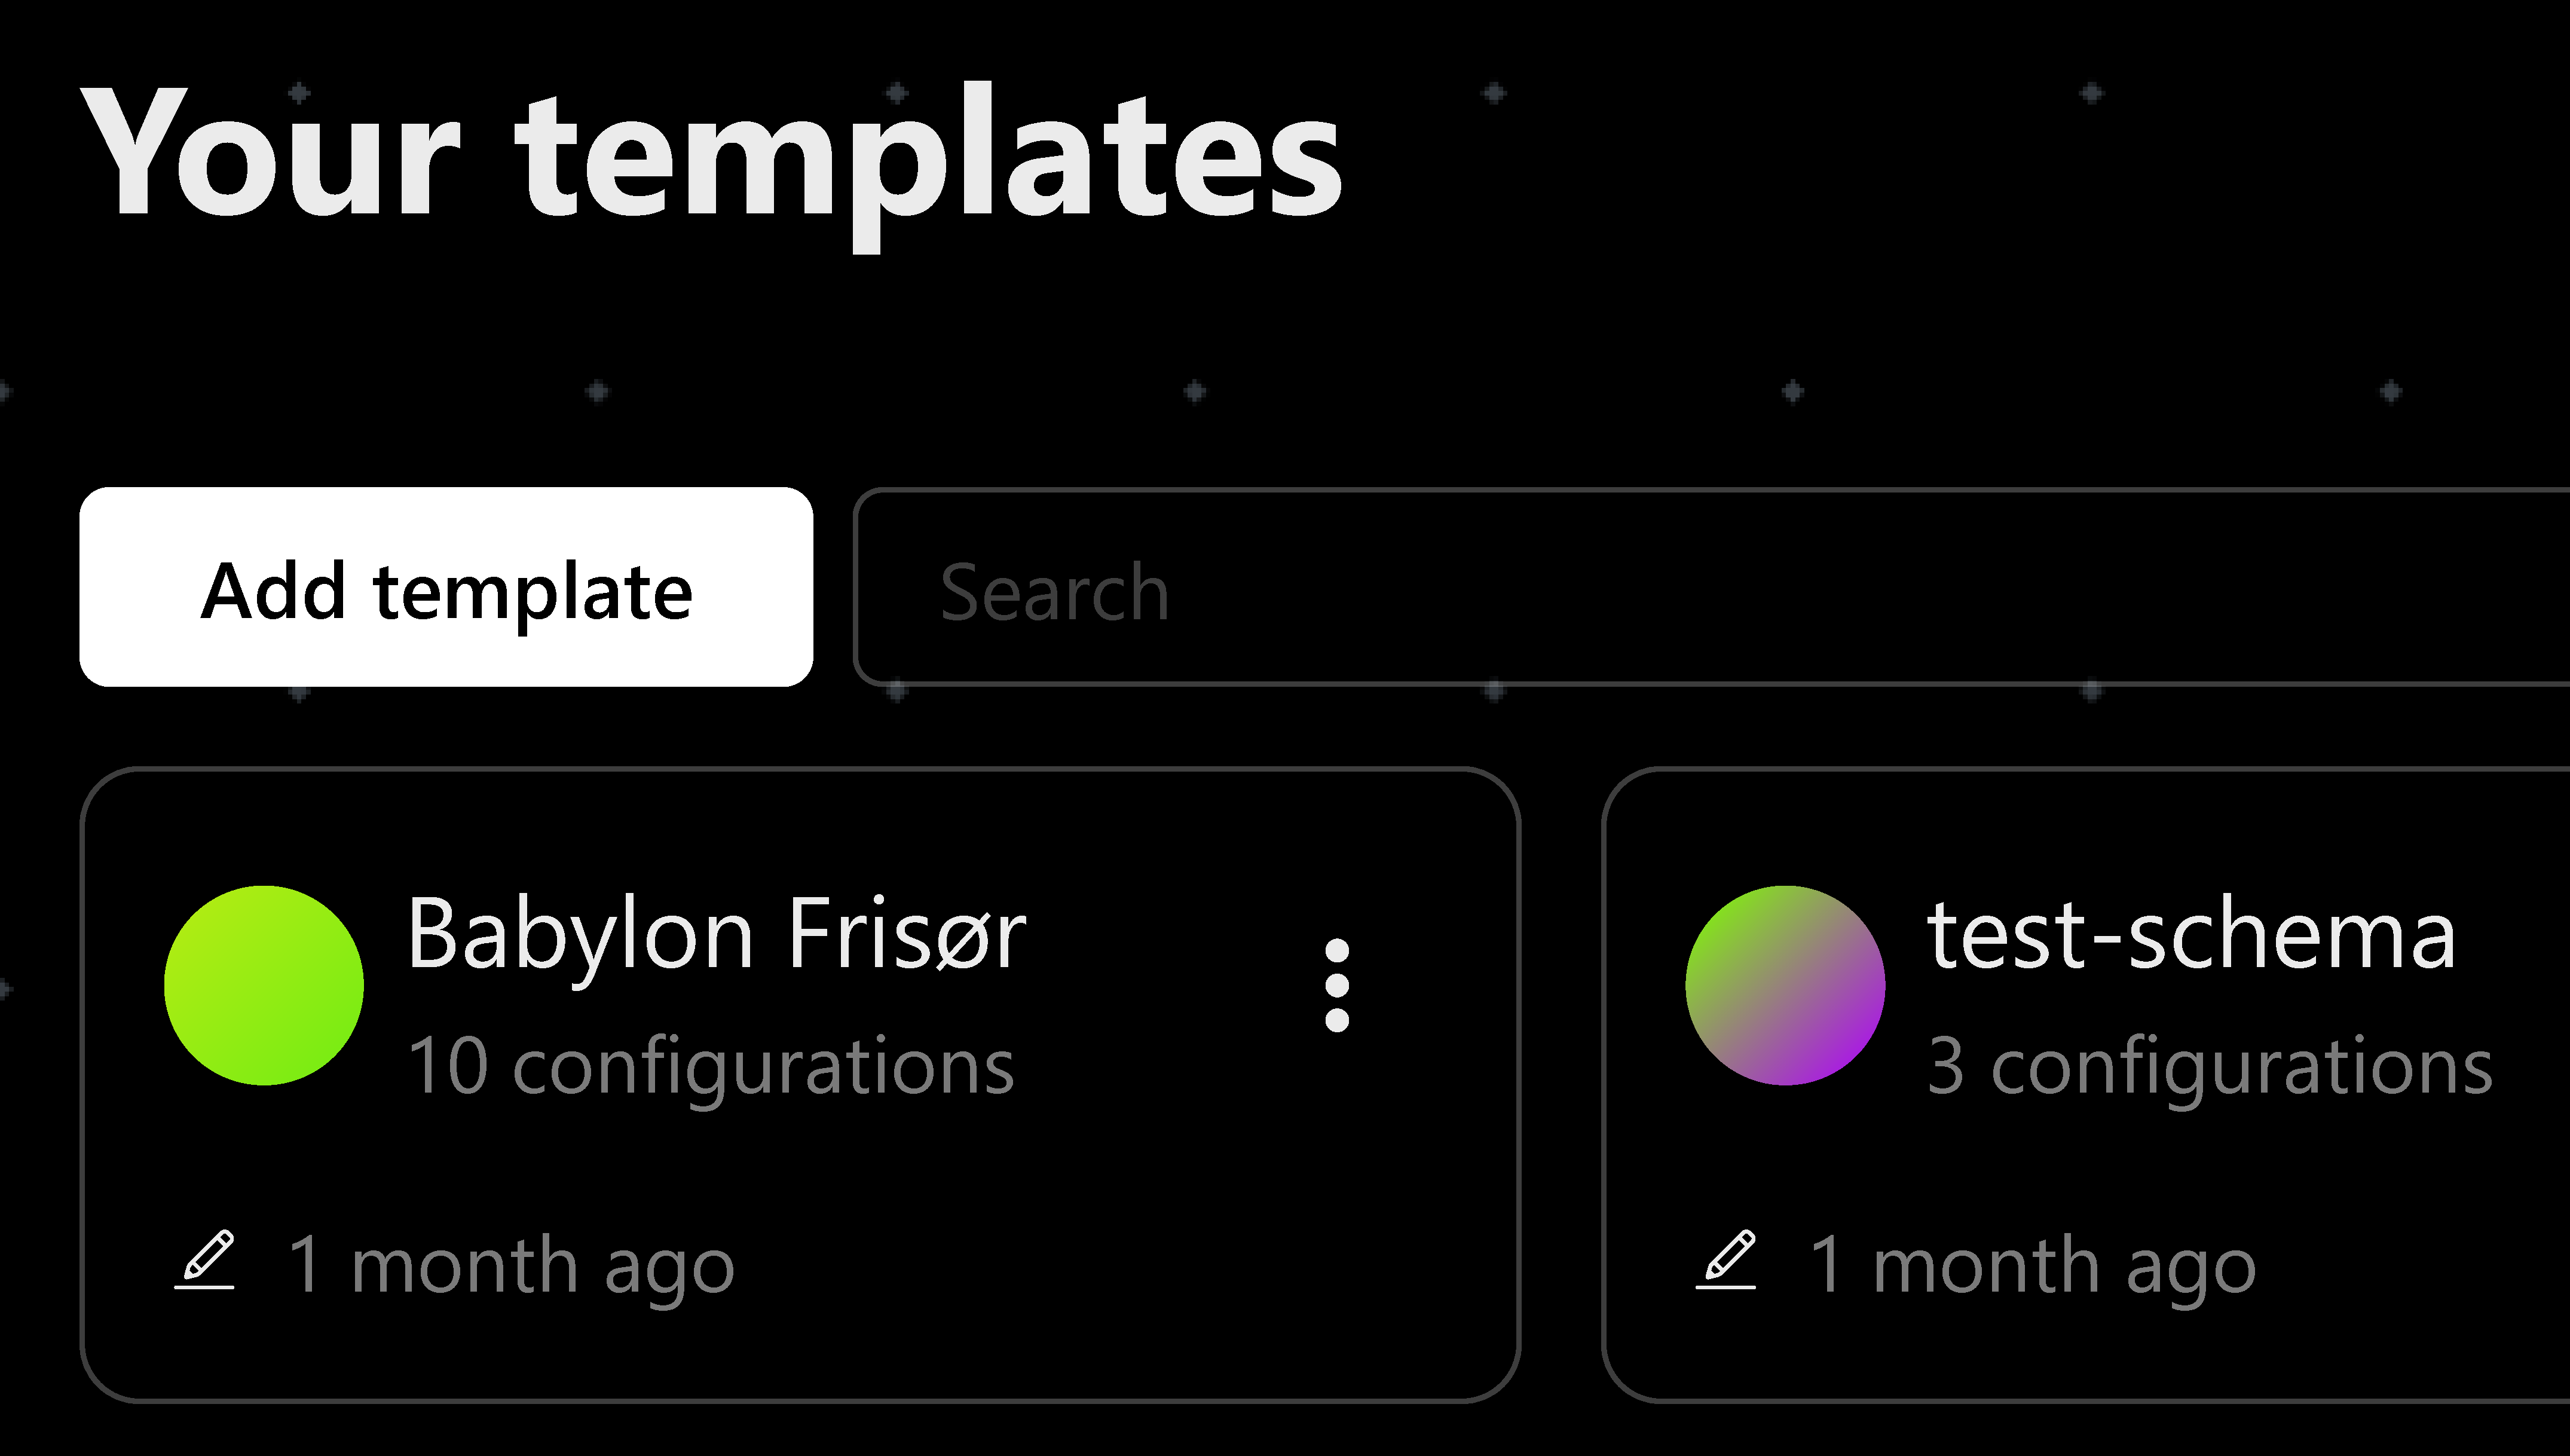
\includegraphics[width=1.\linewidth]{Figures/templates-page/add-template-button.pdf}
   \end{minipage}
   \hspace{0.2cm}
   \begin{minipage}{0.3\textwidth}
     \centering
     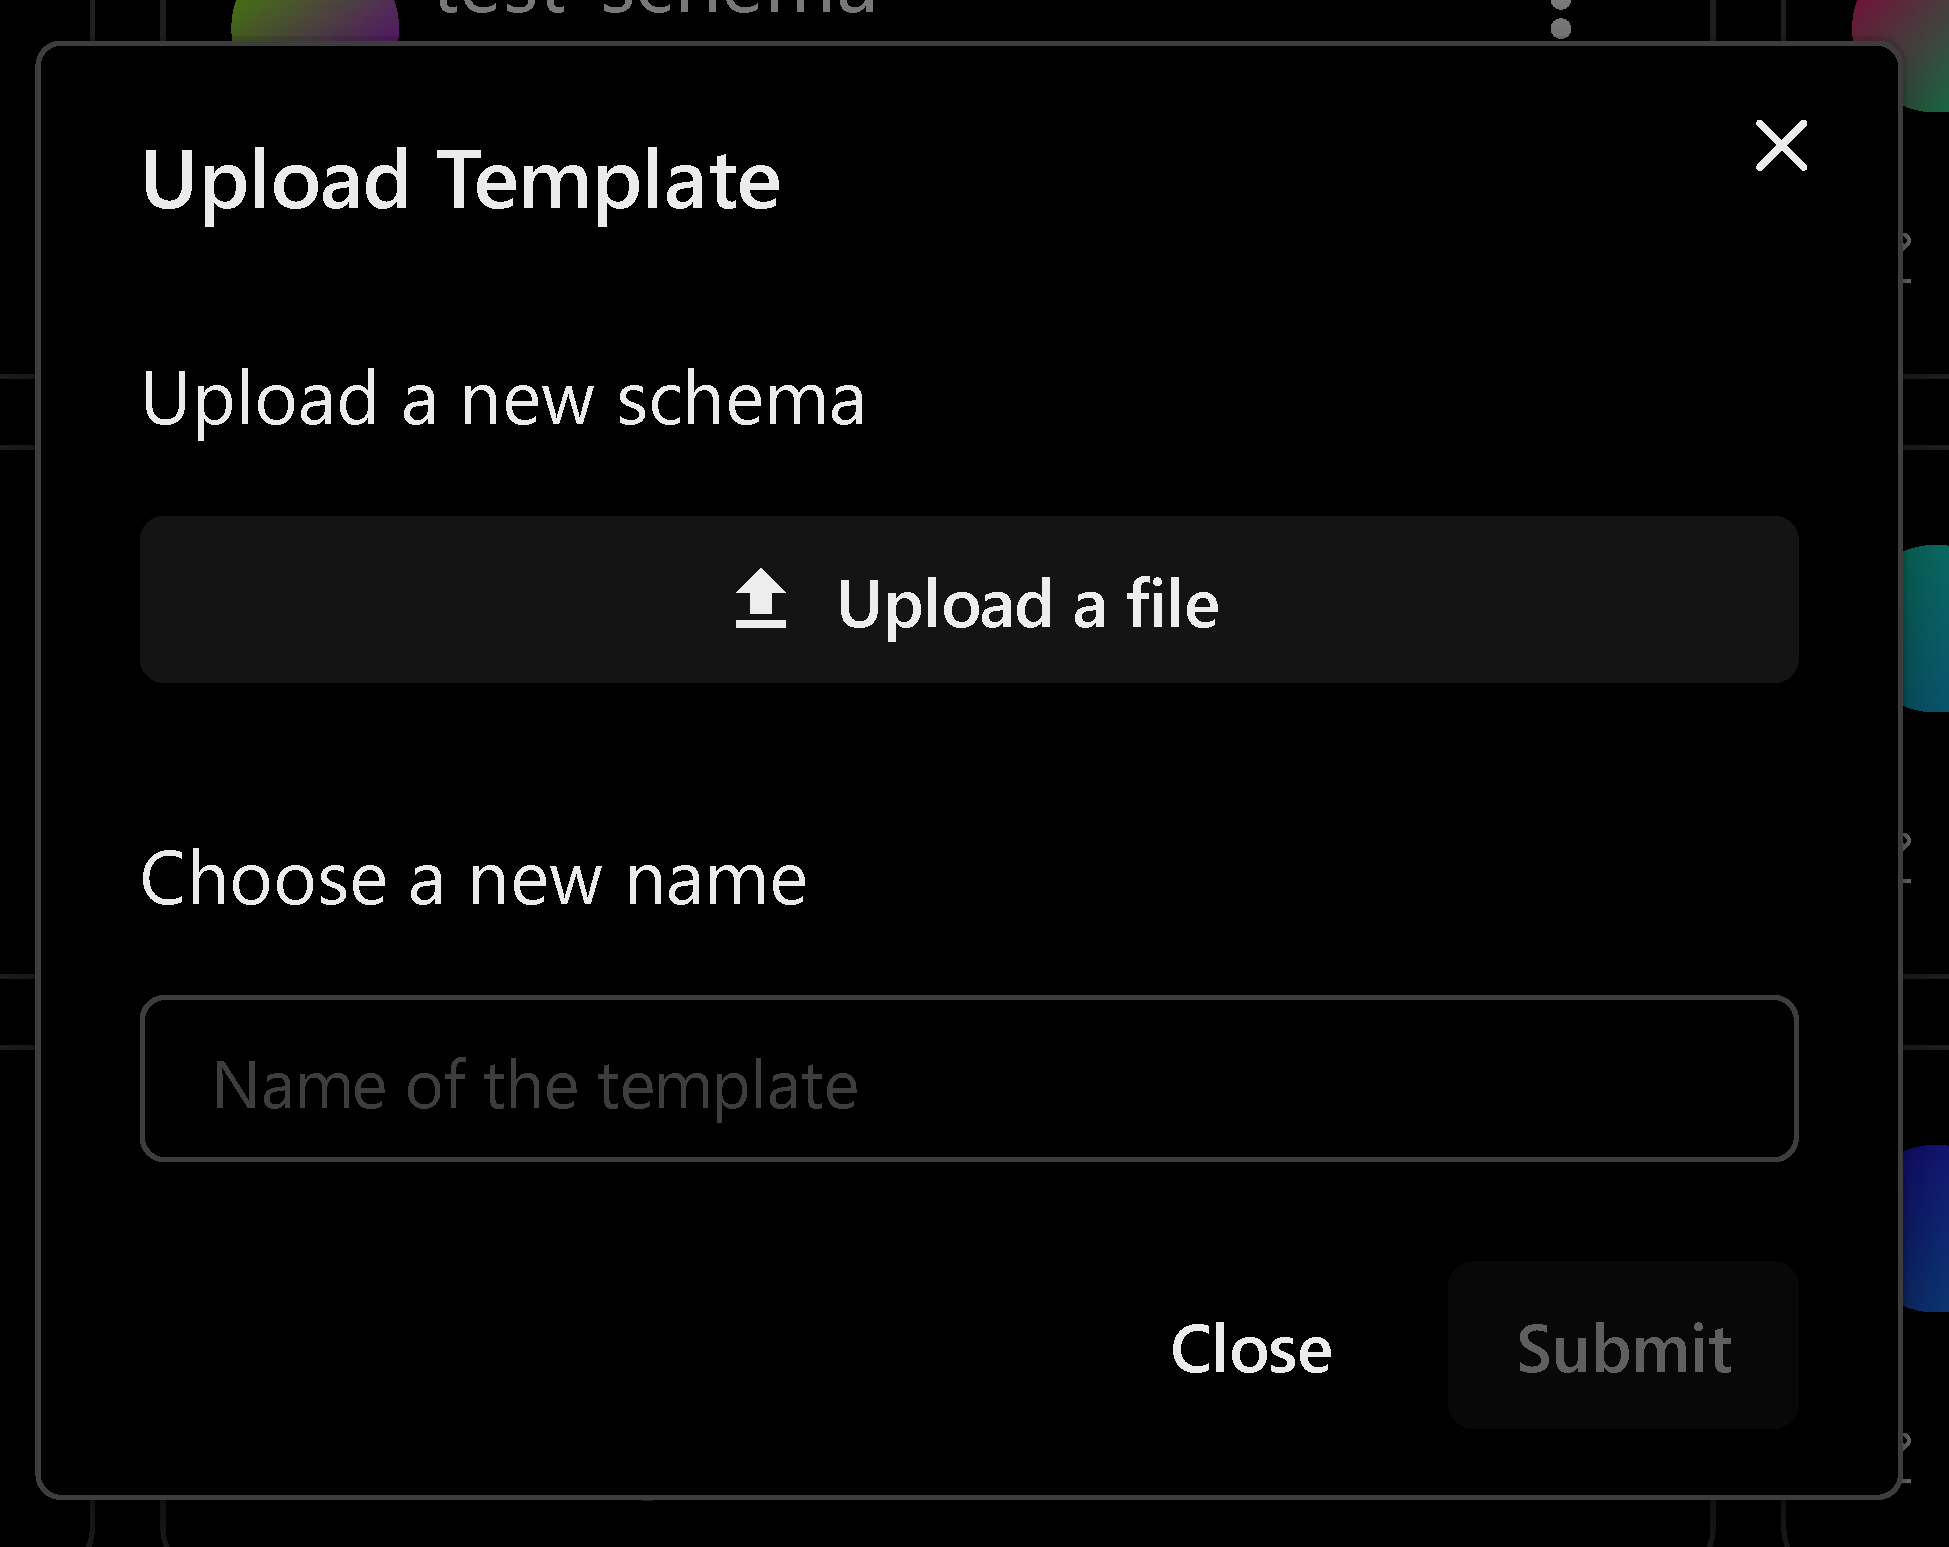
\includegraphics[width=.9\linewidth]{Figures/templates-page/add-template-dialog.pdf}
   \end{minipage}
   \hspace{0.04cm}
   \begin{minipage}{0.25\textwidth}
     \centering
     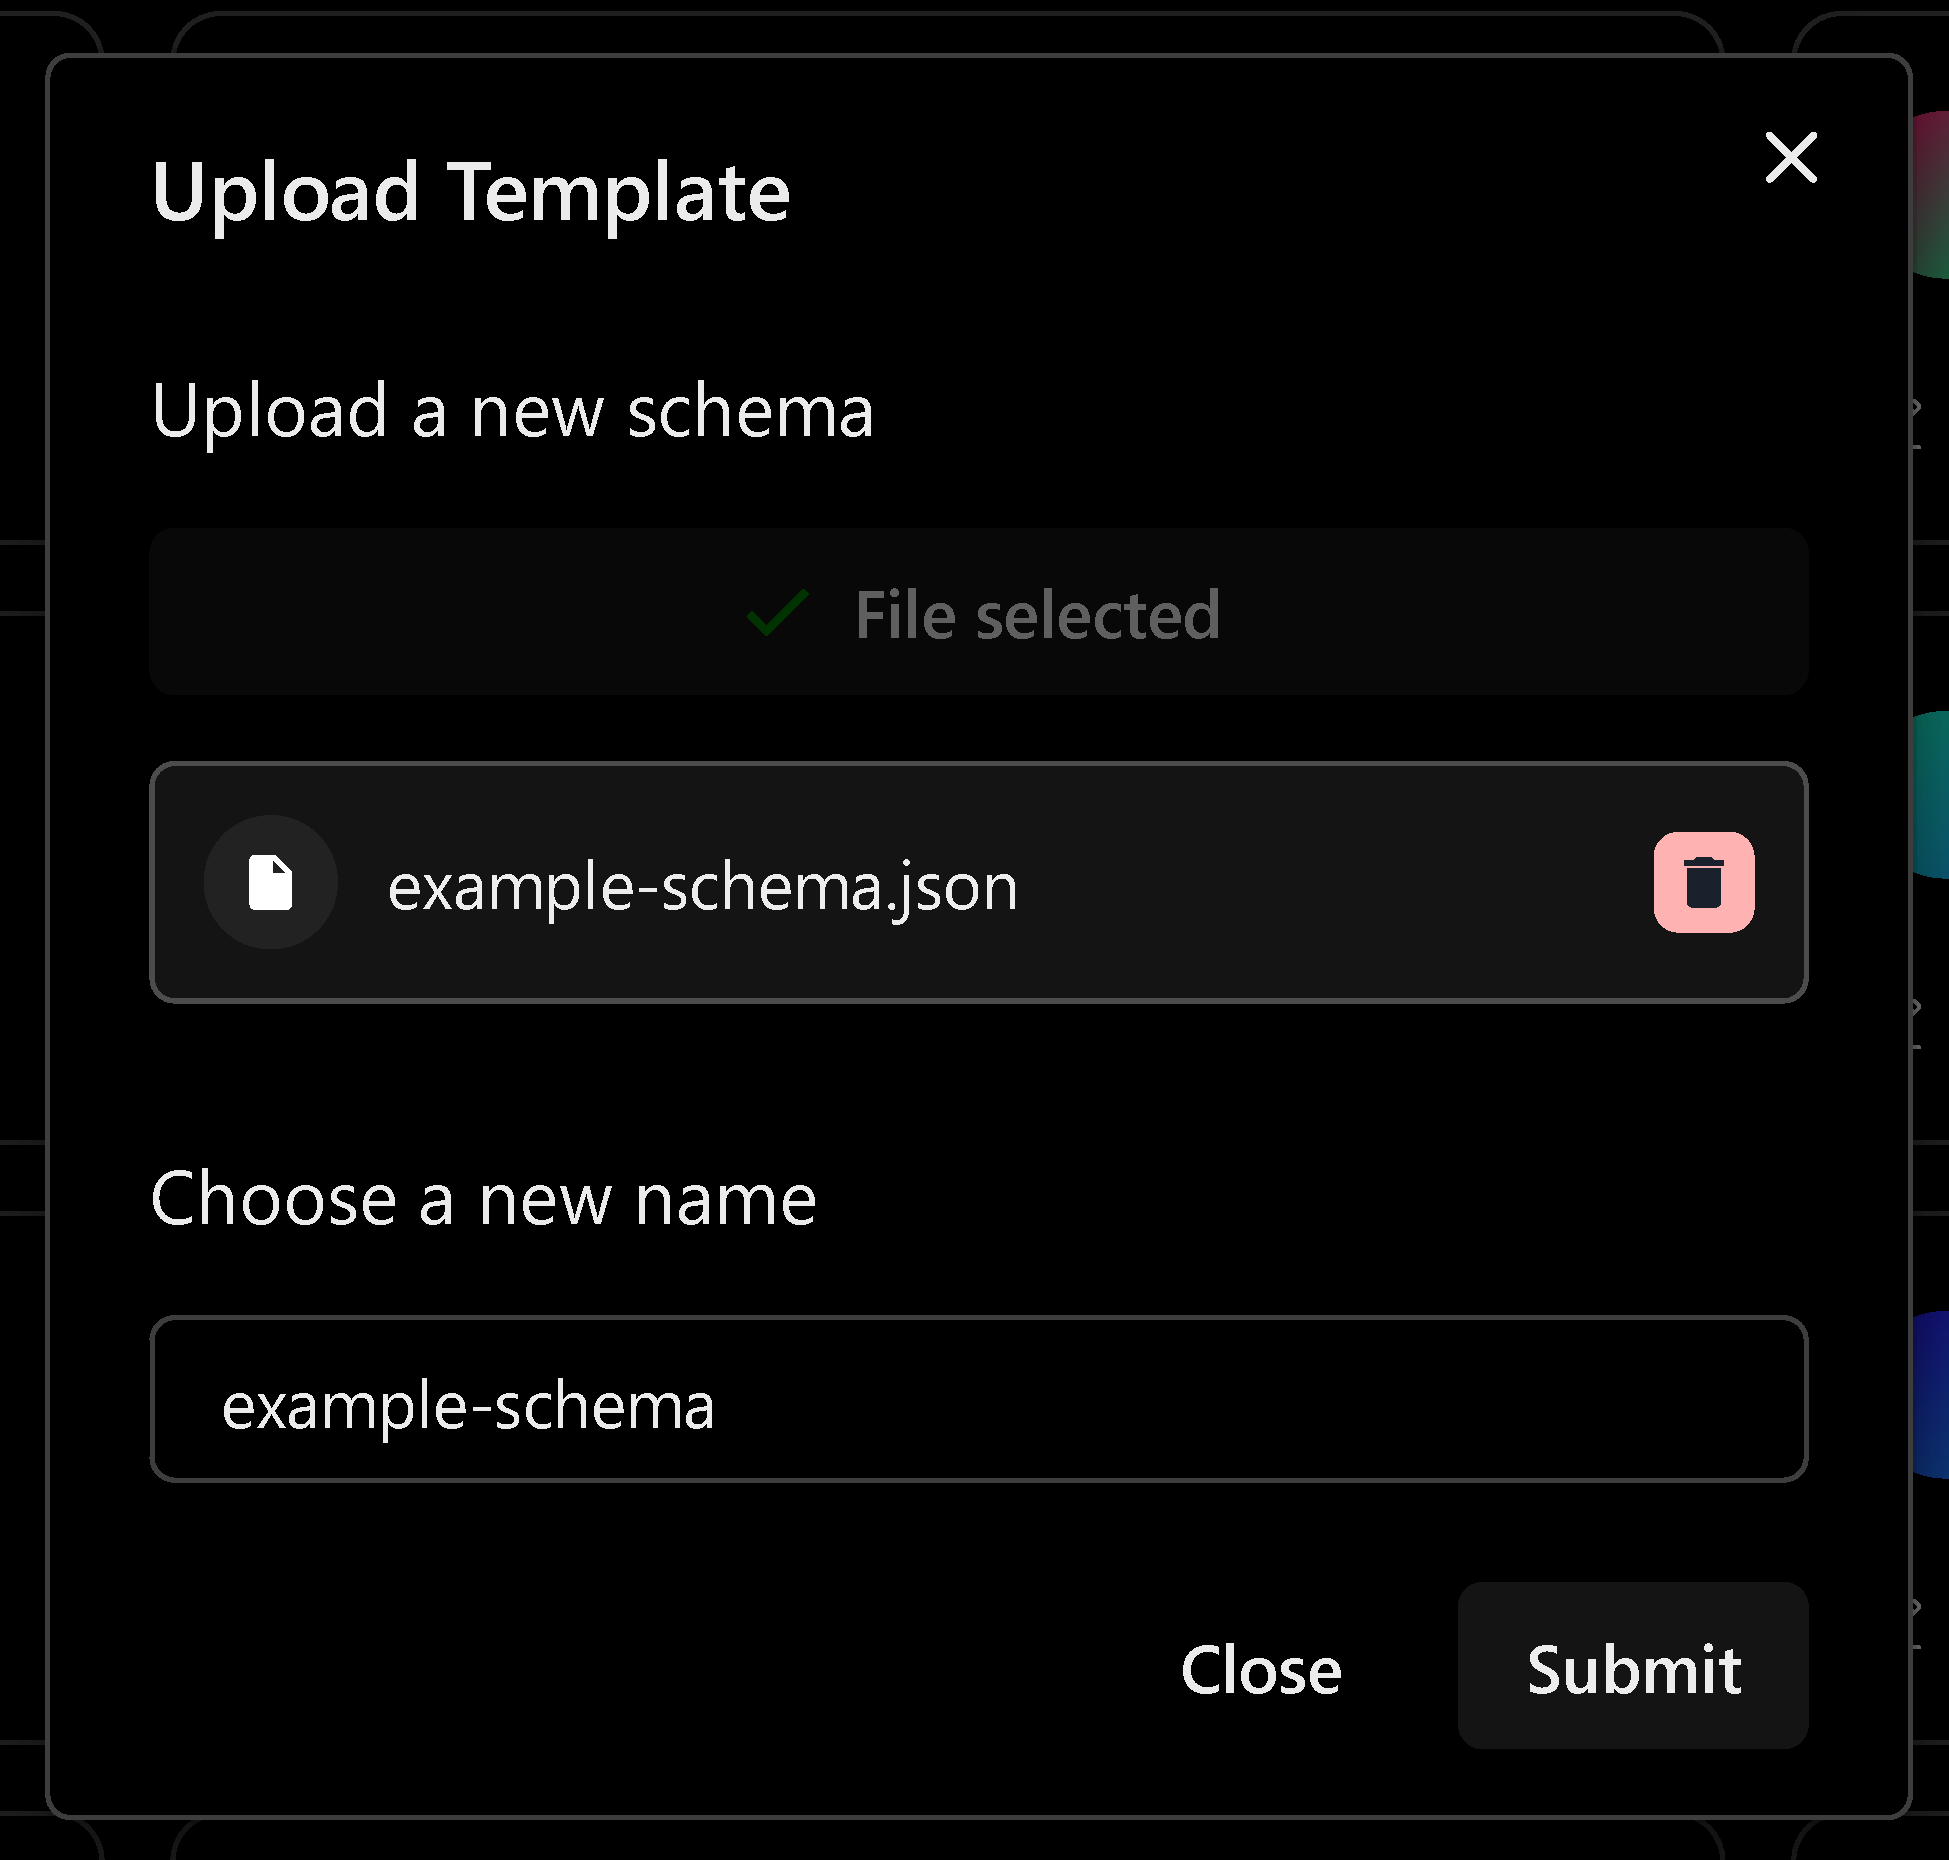
\includegraphics[width=.9\linewidth]{Figures/templates-page/file-selected.pdf}
   \end{minipage}
   \caption[Template (JSON schema) upload process]{This figure illustrates the process of uploading a template (JSON schema).}
   \label{adding:template}
\end{figure}


\subsection{Adding a configuration (JSON file)}

When the user opens a template, they are presented with different configurations contained in that template. These are the different JSON files that the user has uploaded and want to verify the content of. The process of uploading a new configuration is similar to that of adding a template. However, in this case, the user is initially presented with three options to choose from. See \autoref{adding:configuration-start} and \autoref{adding:configuration} for visual representation of the steps. The first option is to create a new configuration from scratch. This will create an empty JSON file, where the user can add all the necessary fields. The second option is to copy JSON content from an already existing configuration, while the last option is to upload a JSON file. 

% This picture is probably too small to be seen, a cropped version is included in the folder
% It is actually not, we printed it out
\begin{figure}[!ht]
   \begin{minipage}{1\textwidth}
     \centering
     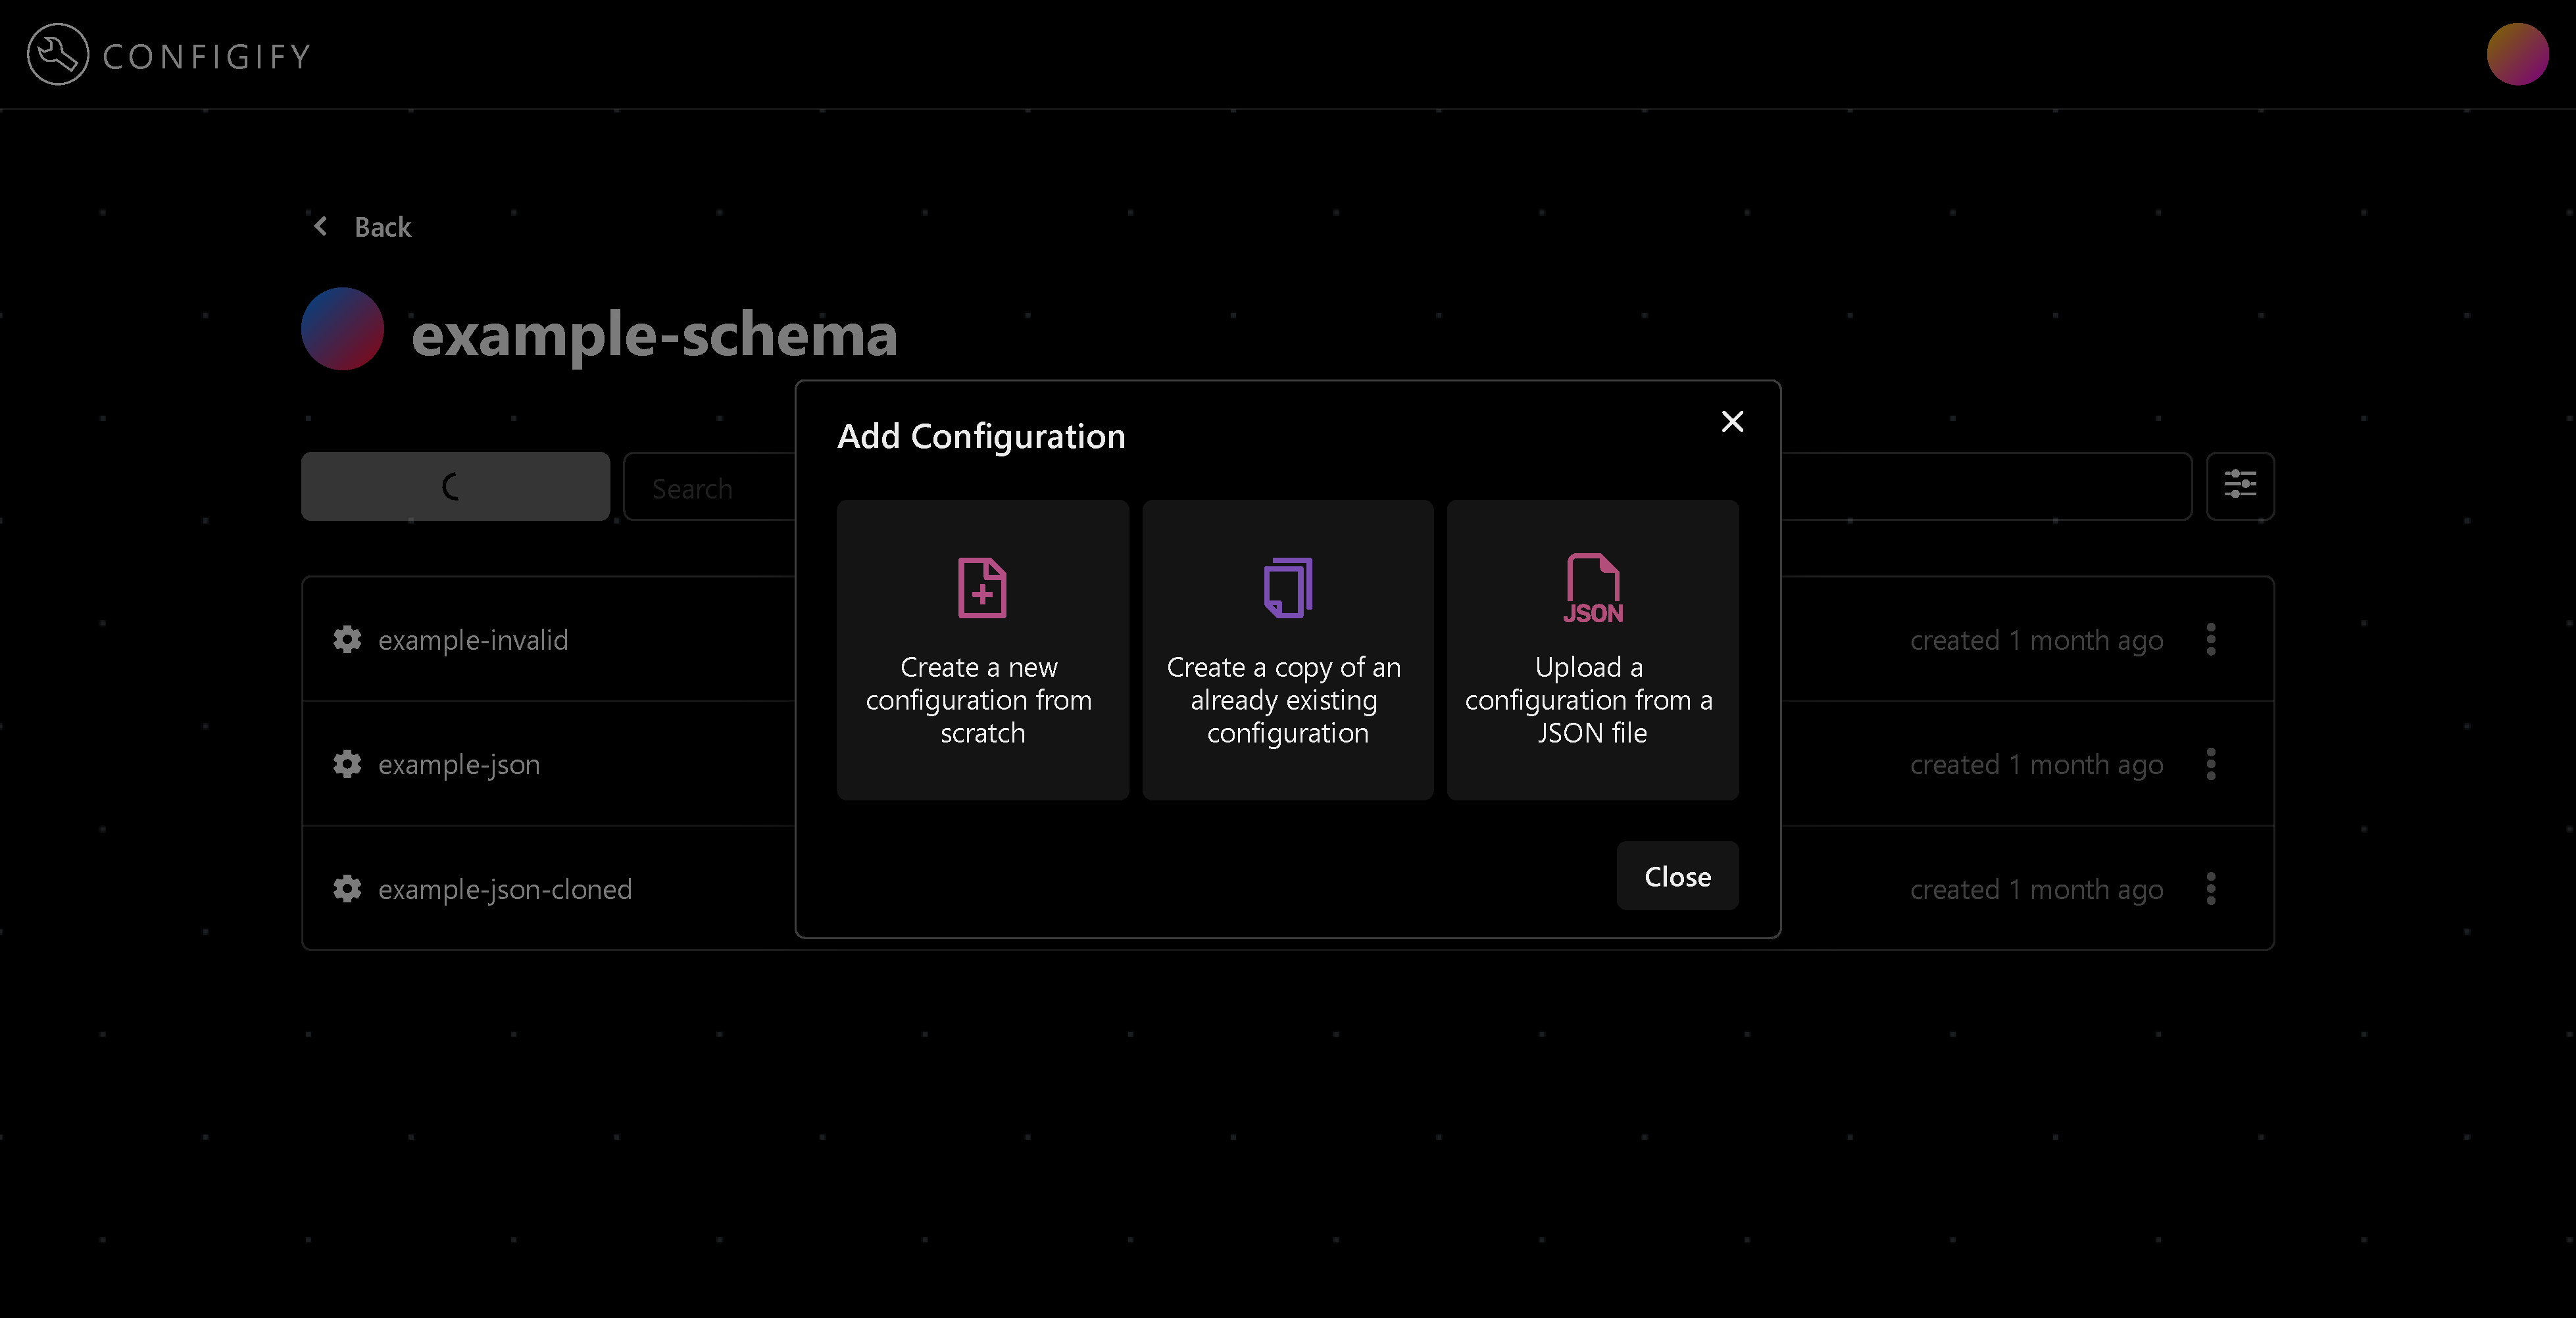
\includegraphics[width=.85\textwidth]{Figures/configurations-page/add-config.pdf}
     \caption[Add configuration dialog]{Figure showing the dialog for adding a new configuration}
     \label{adding:configuration-start}
   \end{minipage}\hfill
\end{figure}

\begin{figure}[!ht]
   \begin{minipage}{0.4\textwidth}
     \centering
     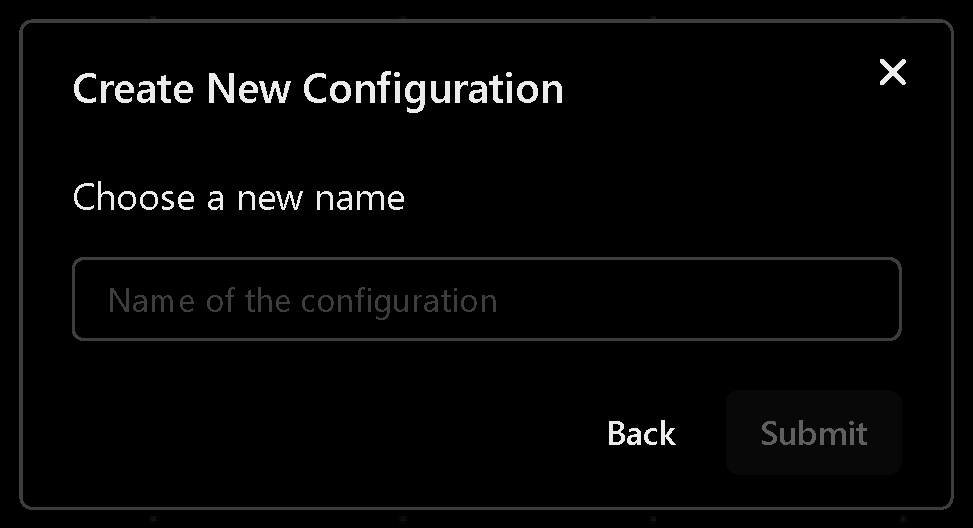
\includegraphics[width=.9\linewidth]{Figures/configurations-page/create-new-crop.pdf}
   \end{minipage}
   \hspace{0.01cm}
   \begin{minipage}{0.27\textwidth}
     \centering
     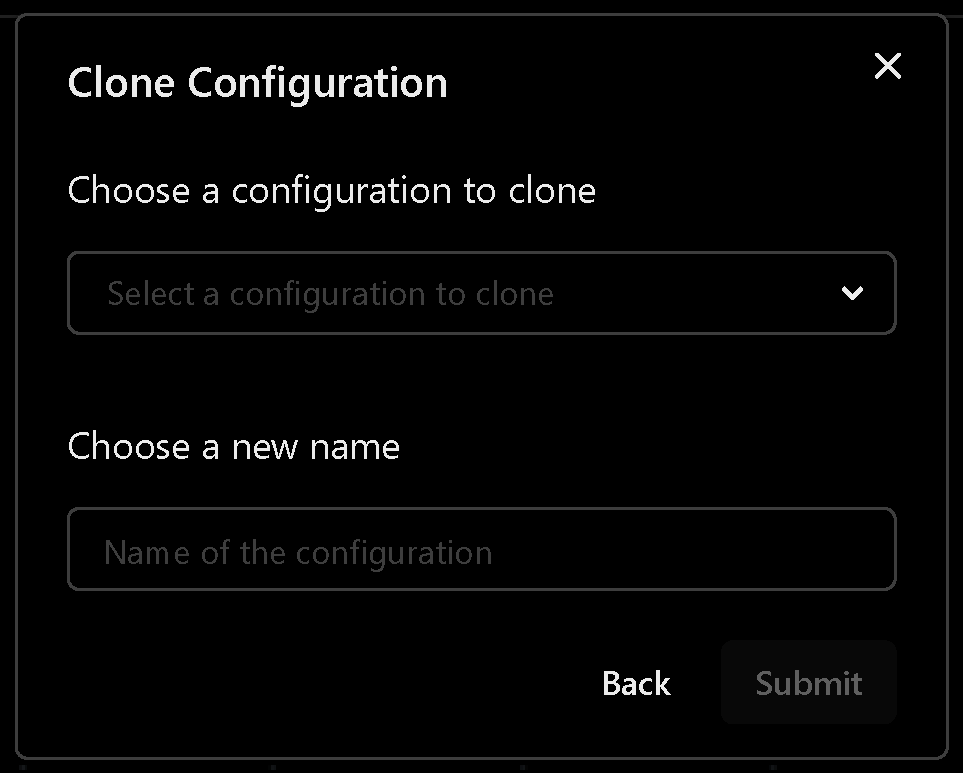
\includegraphics[width=.9\linewidth]{Figures/configurations-page/clone-crop.pdf}
   \end{minipage}
   \hspace{0.05cm}
   \begin{minipage}{0.275\textwidth}
     \centering
     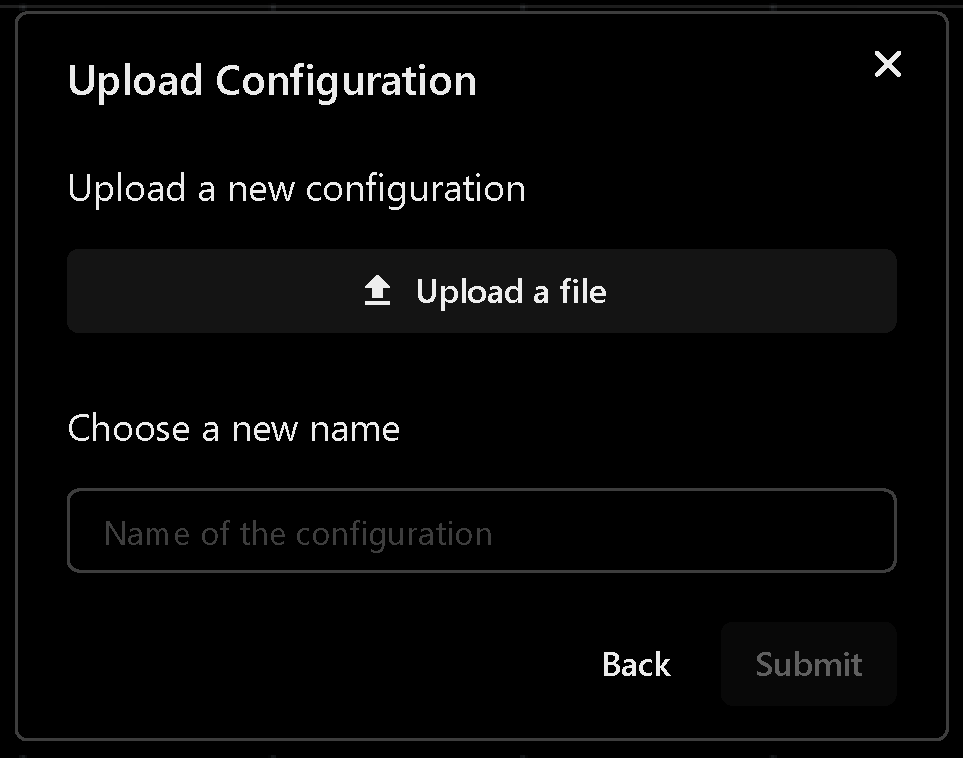
\includegraphics[width=.9\linewidth]{Figures/configurations-page/upload-crop.pdf}
   \end{minipage}
   \caption[Three ways to add a configuration]{A figure showing the 3 ways to add a configuration. The different dialogs are displayed upon selecting the corresponding option from \autoref{adding:configuration-start}
   }
   \label{adding:configuration}
\end{figure}

\subsection{Browsing configurations}

When the user clicks on a template they are directed to the page of that template. One will then be able to browse through all the configurations of that template. The configurations are sorted by last modified, the most recent modified will appear on the top.

\subsubsection{Search}

Due to the uncertainty related to the number of configurations to be added, it could potentially be hard to locate the specific configuration the user is looking for. To address this concern, we implemented a search functionality within to allow users to find specific configurations. Our approach utilized a simple search algorithm that involved checking if the search term appeared within the title of the template. The search algorithm was also case-insensitive to improve usability. The same is also used for the templates page. See \autoref{search:configuration} for a simple demonstration of the search functionality.

\begin{figure}[!ht]
   \begin{minipage}{1\textwidth}
    \centering
    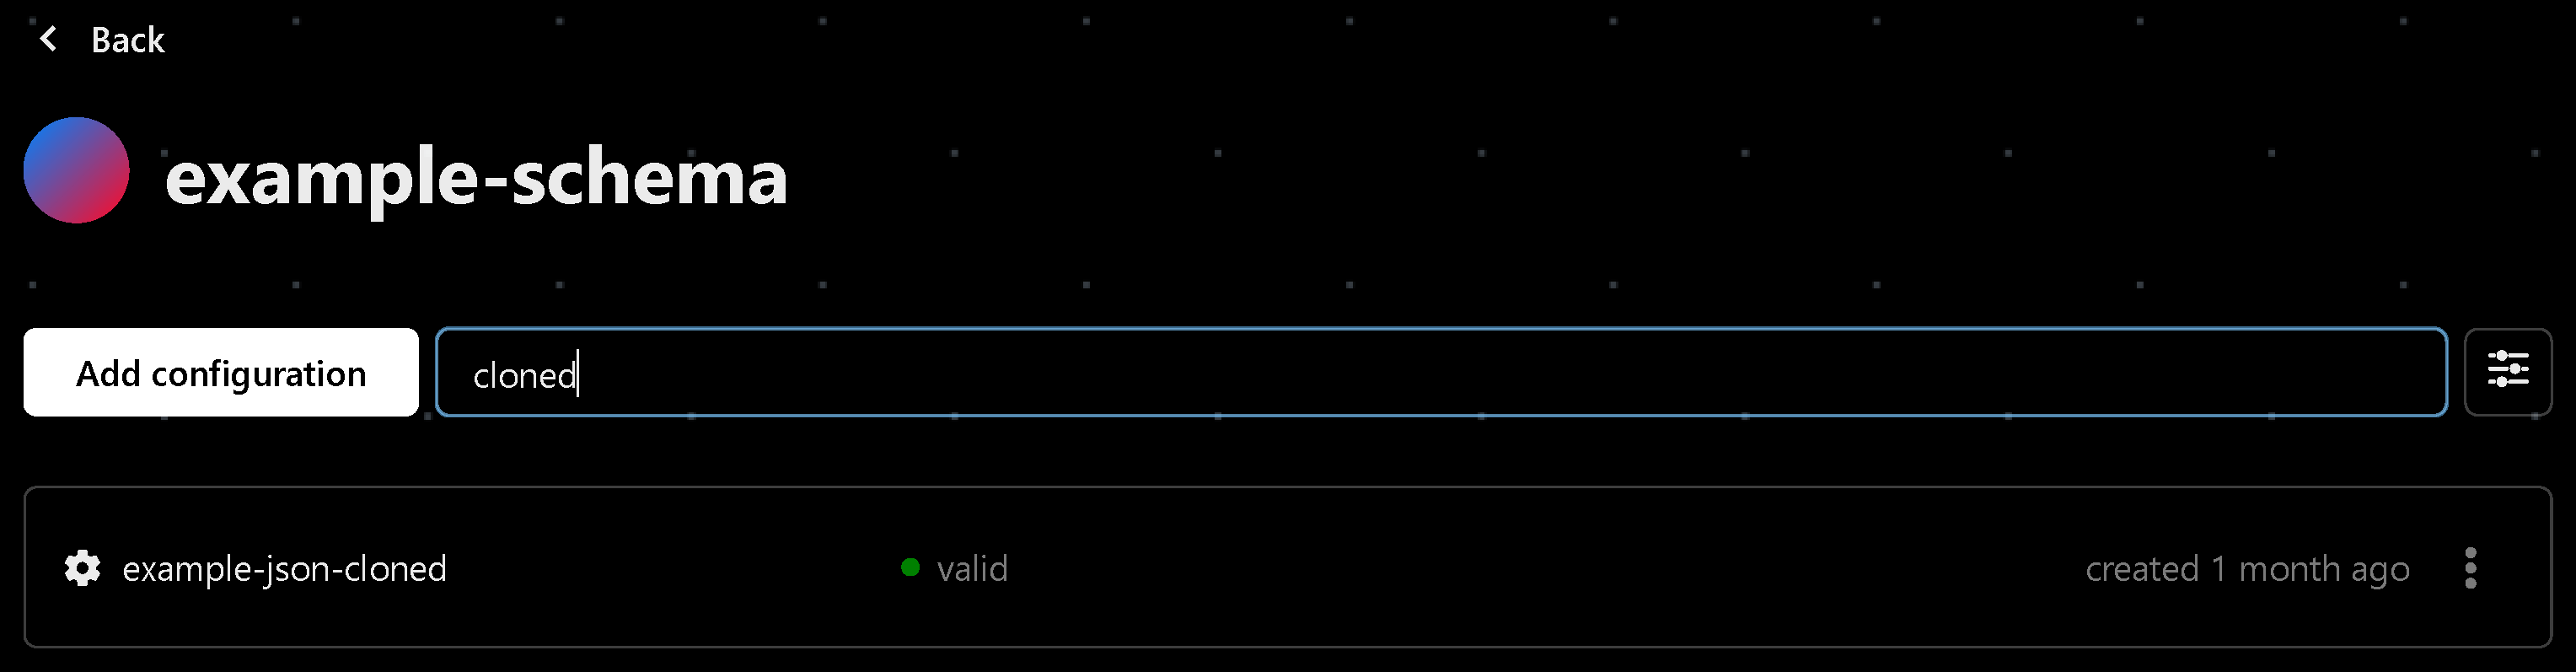
\includegraphics[width=.85\textwidth]{Figures/configurations-page/search-crop.pdf}
     \caption[Configuration search demo]{Search functionality demonstration. A query for the term ‘cloned’ yielded a single result.}
     \label{search:configuration}
   \end{minipage}\hfill
\end{figure}

\subsubsection{Filter}

An important part of the application is the ability to update a schema. In relations to this, when a schema is updated, all the existing configurations for that template will be re-validated. This means that a lot of the  configurations might be changed to being invalid. To allow the user to quickly find invalid configurations, we created a simple filter, so that the user can switch between displaying all, valid or invalid configurations. The filter button also displays a tiny icon on the button to show which filter is currently selected, see \autoref{filter:configuration} and \autoref{filter-selected:configuration} for a demonstration.


\begin{figure}[!ht]
   \begin{minipage}{1\textwidth}
    \centering
    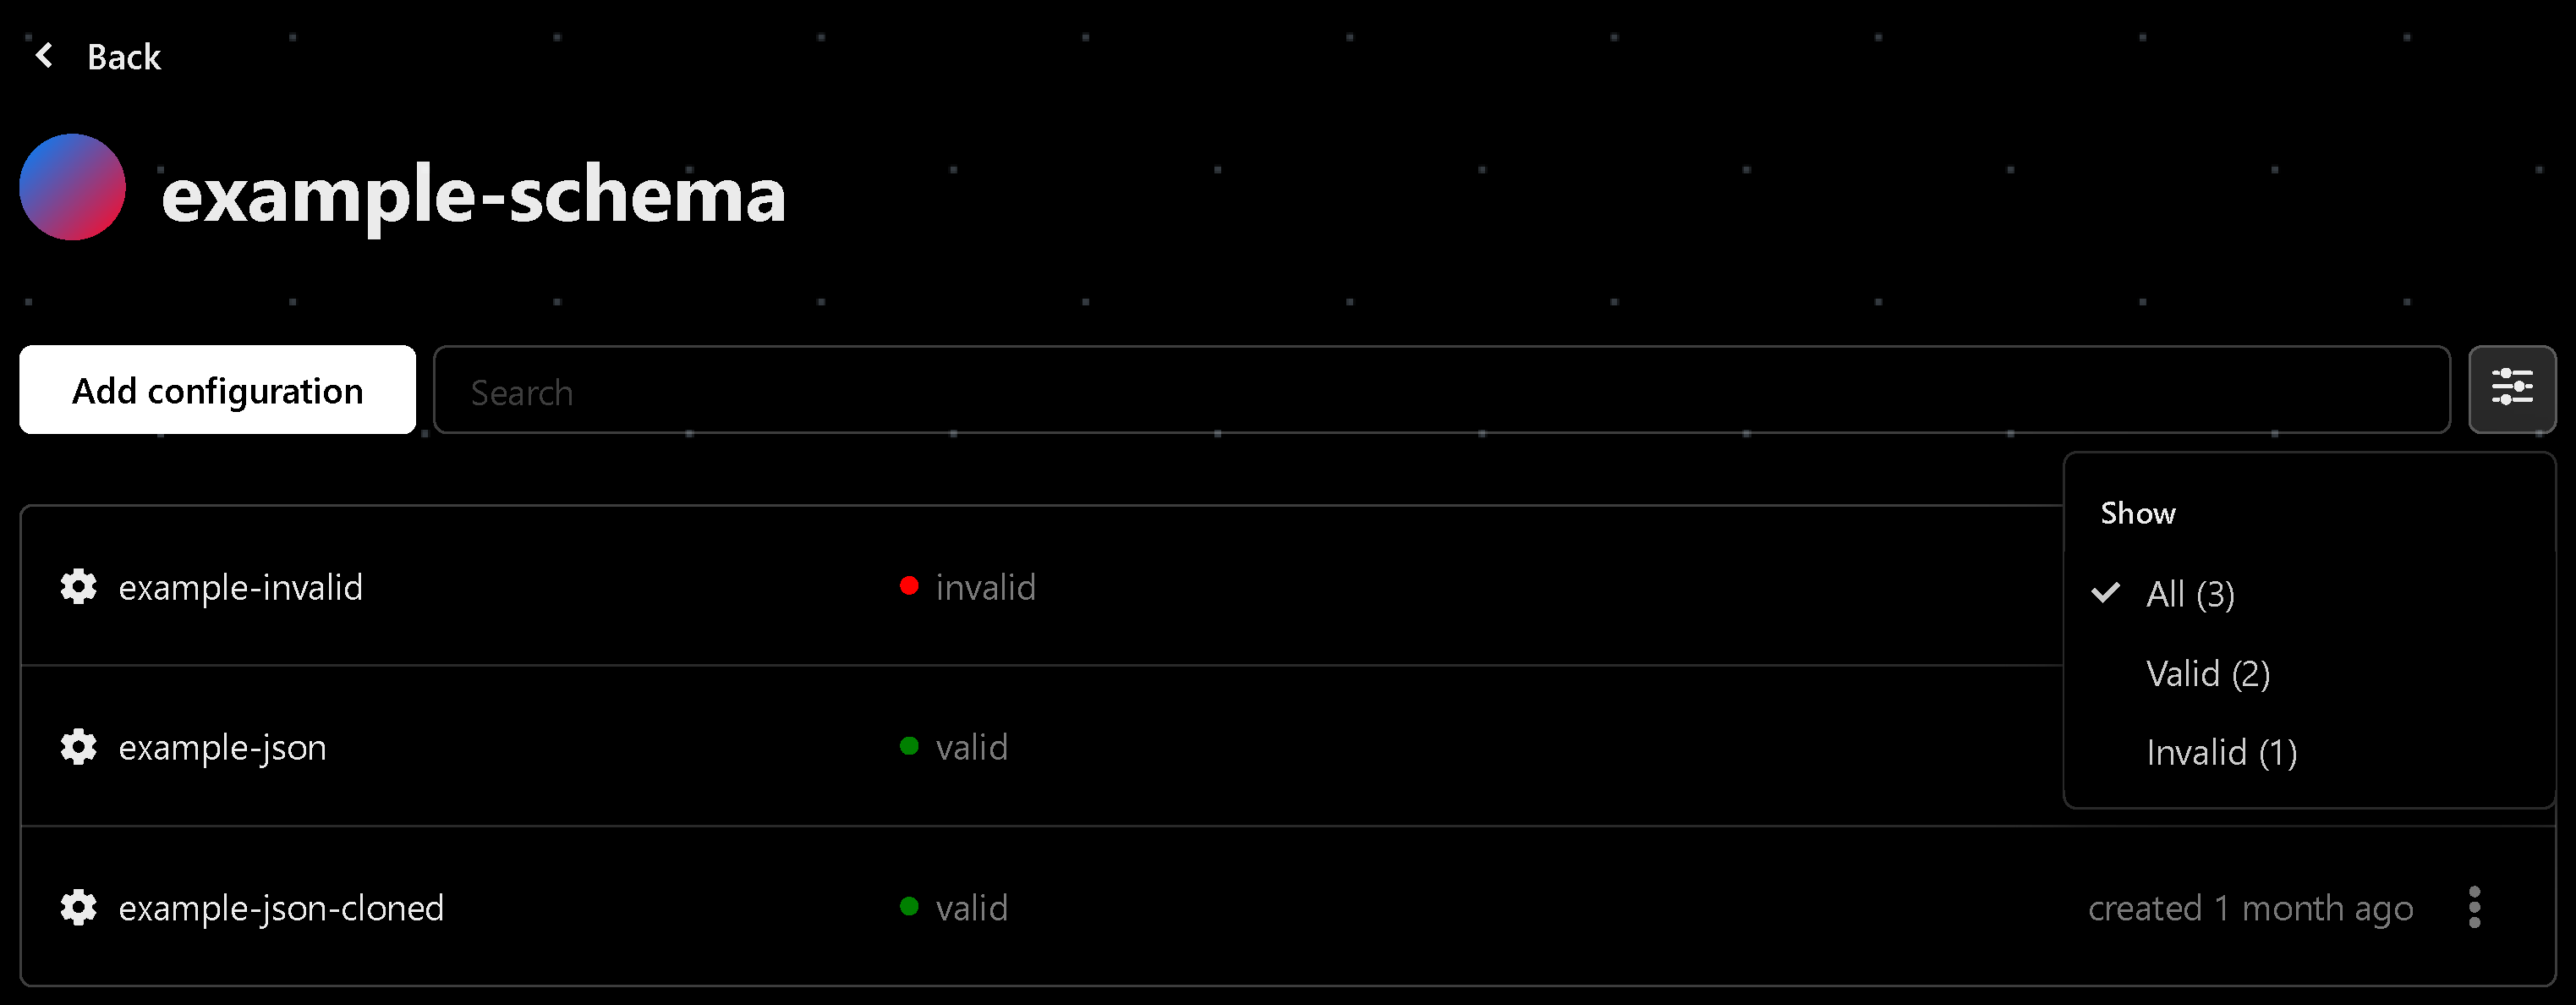
\includegraphics[width=.85\textwidth]{Figures/configurations-page/filter-crop.pdf}
     \caption[Filter dialog]{A figure showing the filter dialog}
     \label{filter:configuration}
   \end{minipage}\hfill
\end{figure}


\begin{figure}[!ht]
   \begin{minipage}{0.73\textwidth}
     \centering
     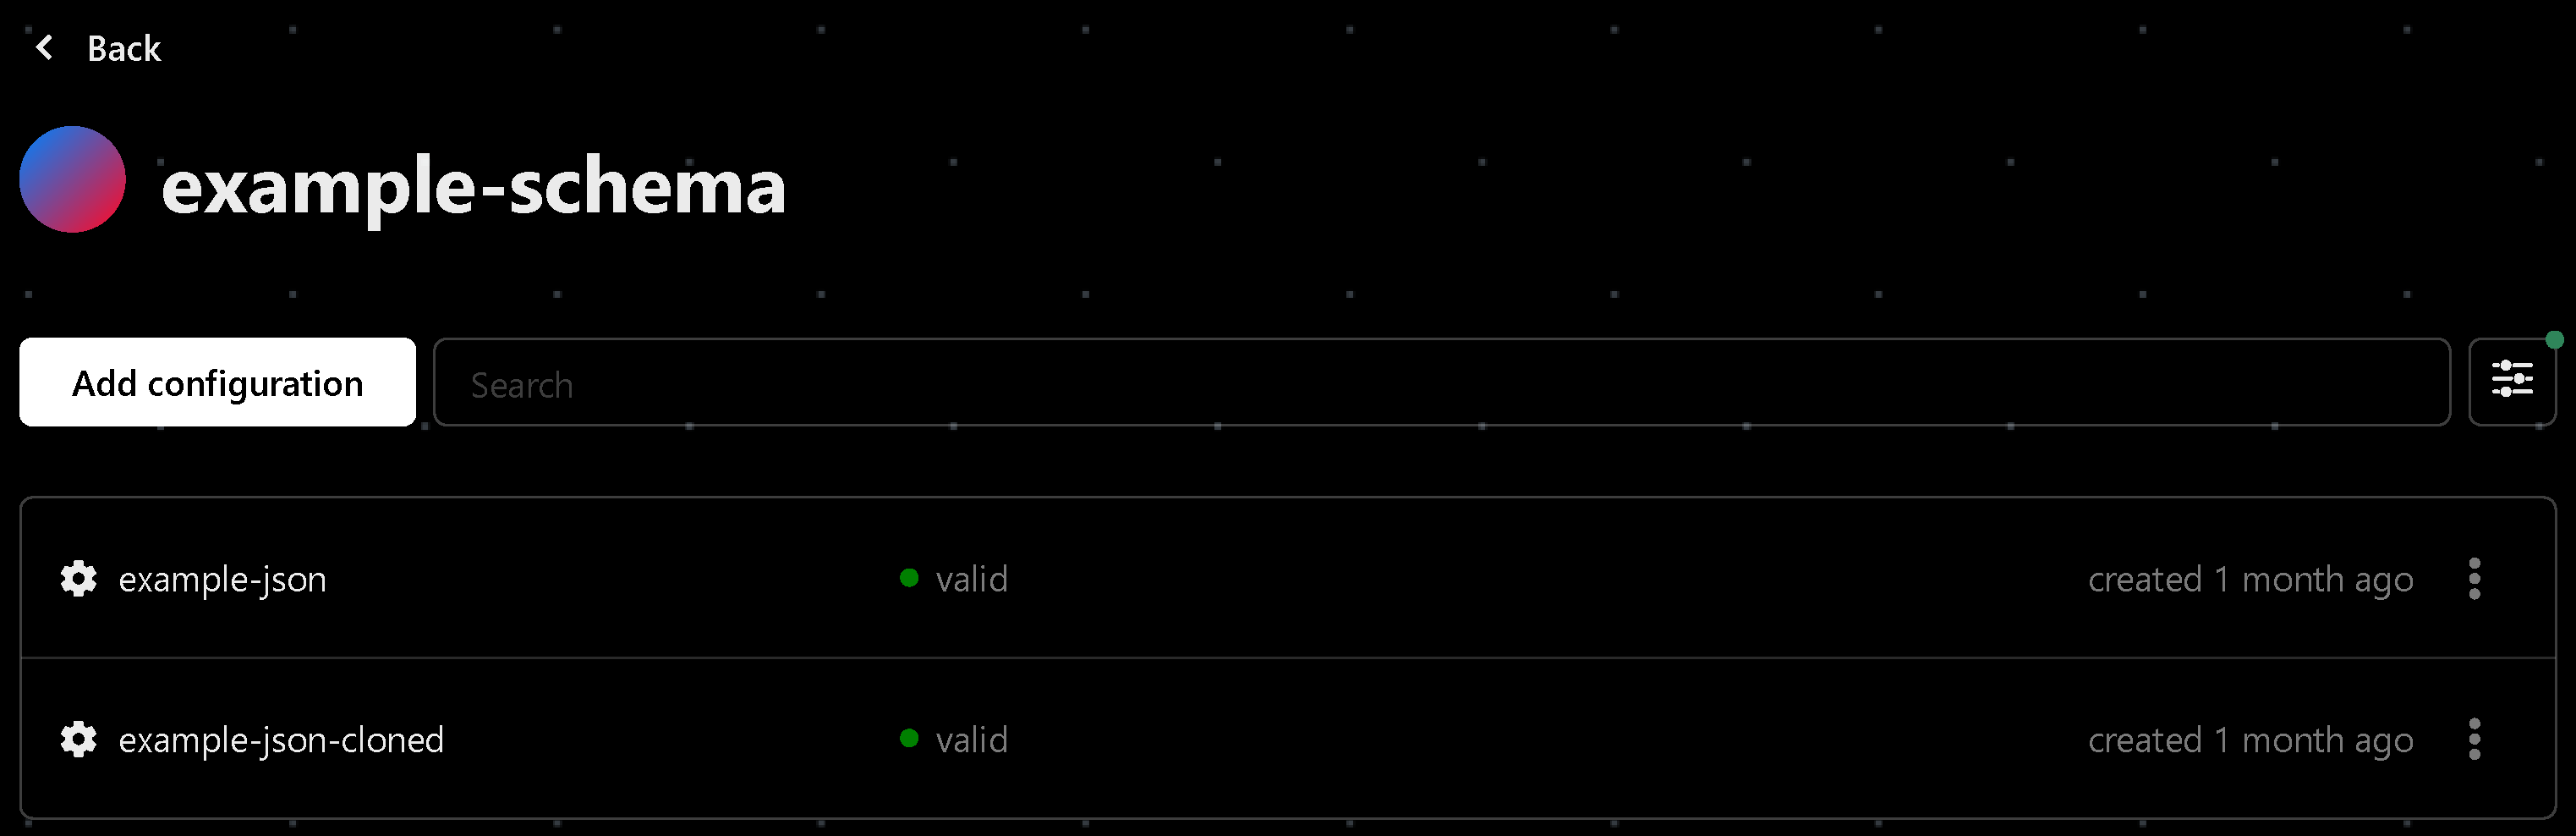
\includegraphics[width=.9\linewidth]{Figures/configurations-page/filter-selected-crop.pdf}
   \end{minipage}
   \hspace{0.01cm}
   \begin{minipage}{0.235\textwidth}
     \centering
     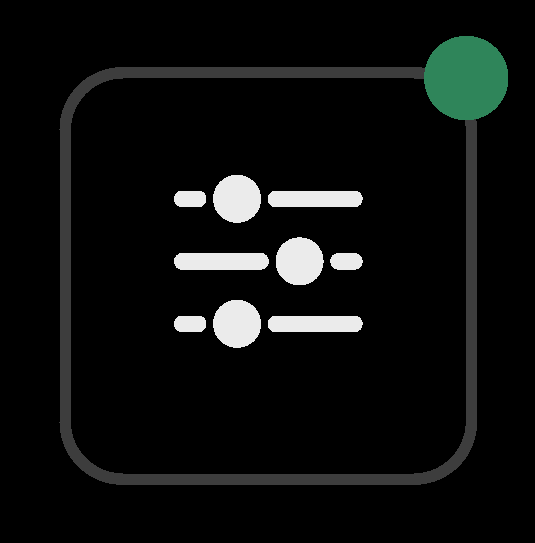
\includegraphics[width=.9\linewidth]{Figures/configurations-page/filter-selected-button-crop.pdf}
   \end{minipage}
   \caption[Filter demo, valid configs only \& filter dot]{A figure demonstrating the filter functionality. On the left, only valid configurations are displayed, while the right figure shows a close-up of the filter button with an added dot to indicate that a filter has been applied}
   \label{filter-selected:configuration}
\end{figure}

\subsubsection{Download}

One of the most important aspects of the application is the ability to download the configurations. When the user modifes a configuration, they need to be able to download it. In the drop-down menu for the different configurations, we added a button that allows the user to download the JSON file. 
\begin{figure}[!ht]
   \begin{minipage}{1\textwidth}
    \centering
    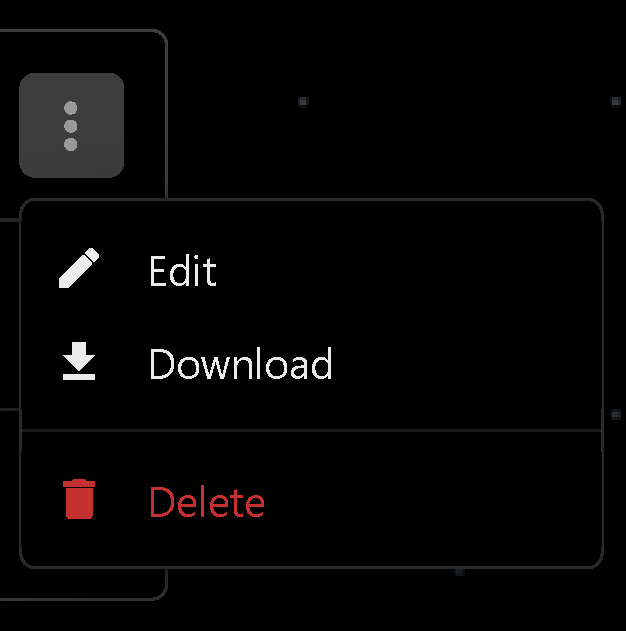
\includegraphics[width=.3\textwidth]{Figures/configurations-page/download-crop.pdf}
     \caption[Config menu - rename, download, delete options]{Configuration menu close-up. The menu displays options to rename, download, and delete the configuration}
     \label{download:configuration}
   \end{minipage}\hfill
\end{figure}

\subsubsection{Other}

In the drop-down menu we also added the option to edit the configuration. This allows the user to change the name, or to upload a new configuration. If the user chooses to upload a new configuration, it will overwrite the existing one.
The final option in the menu is the delete button. This triggers a dialog prompting the user to confirm their intention to delete the configuration. This serves as a safety measure to prevent accidental deletion.

\subsection{Browsing a single configuration}

In the configuration browser, the user will be met with all the inner most objects of the JSON file, see \autoref{browsing:browser}.

\begin{figure}[!ht]
   \begin{minipage}{1\textwidth}
     \centering
     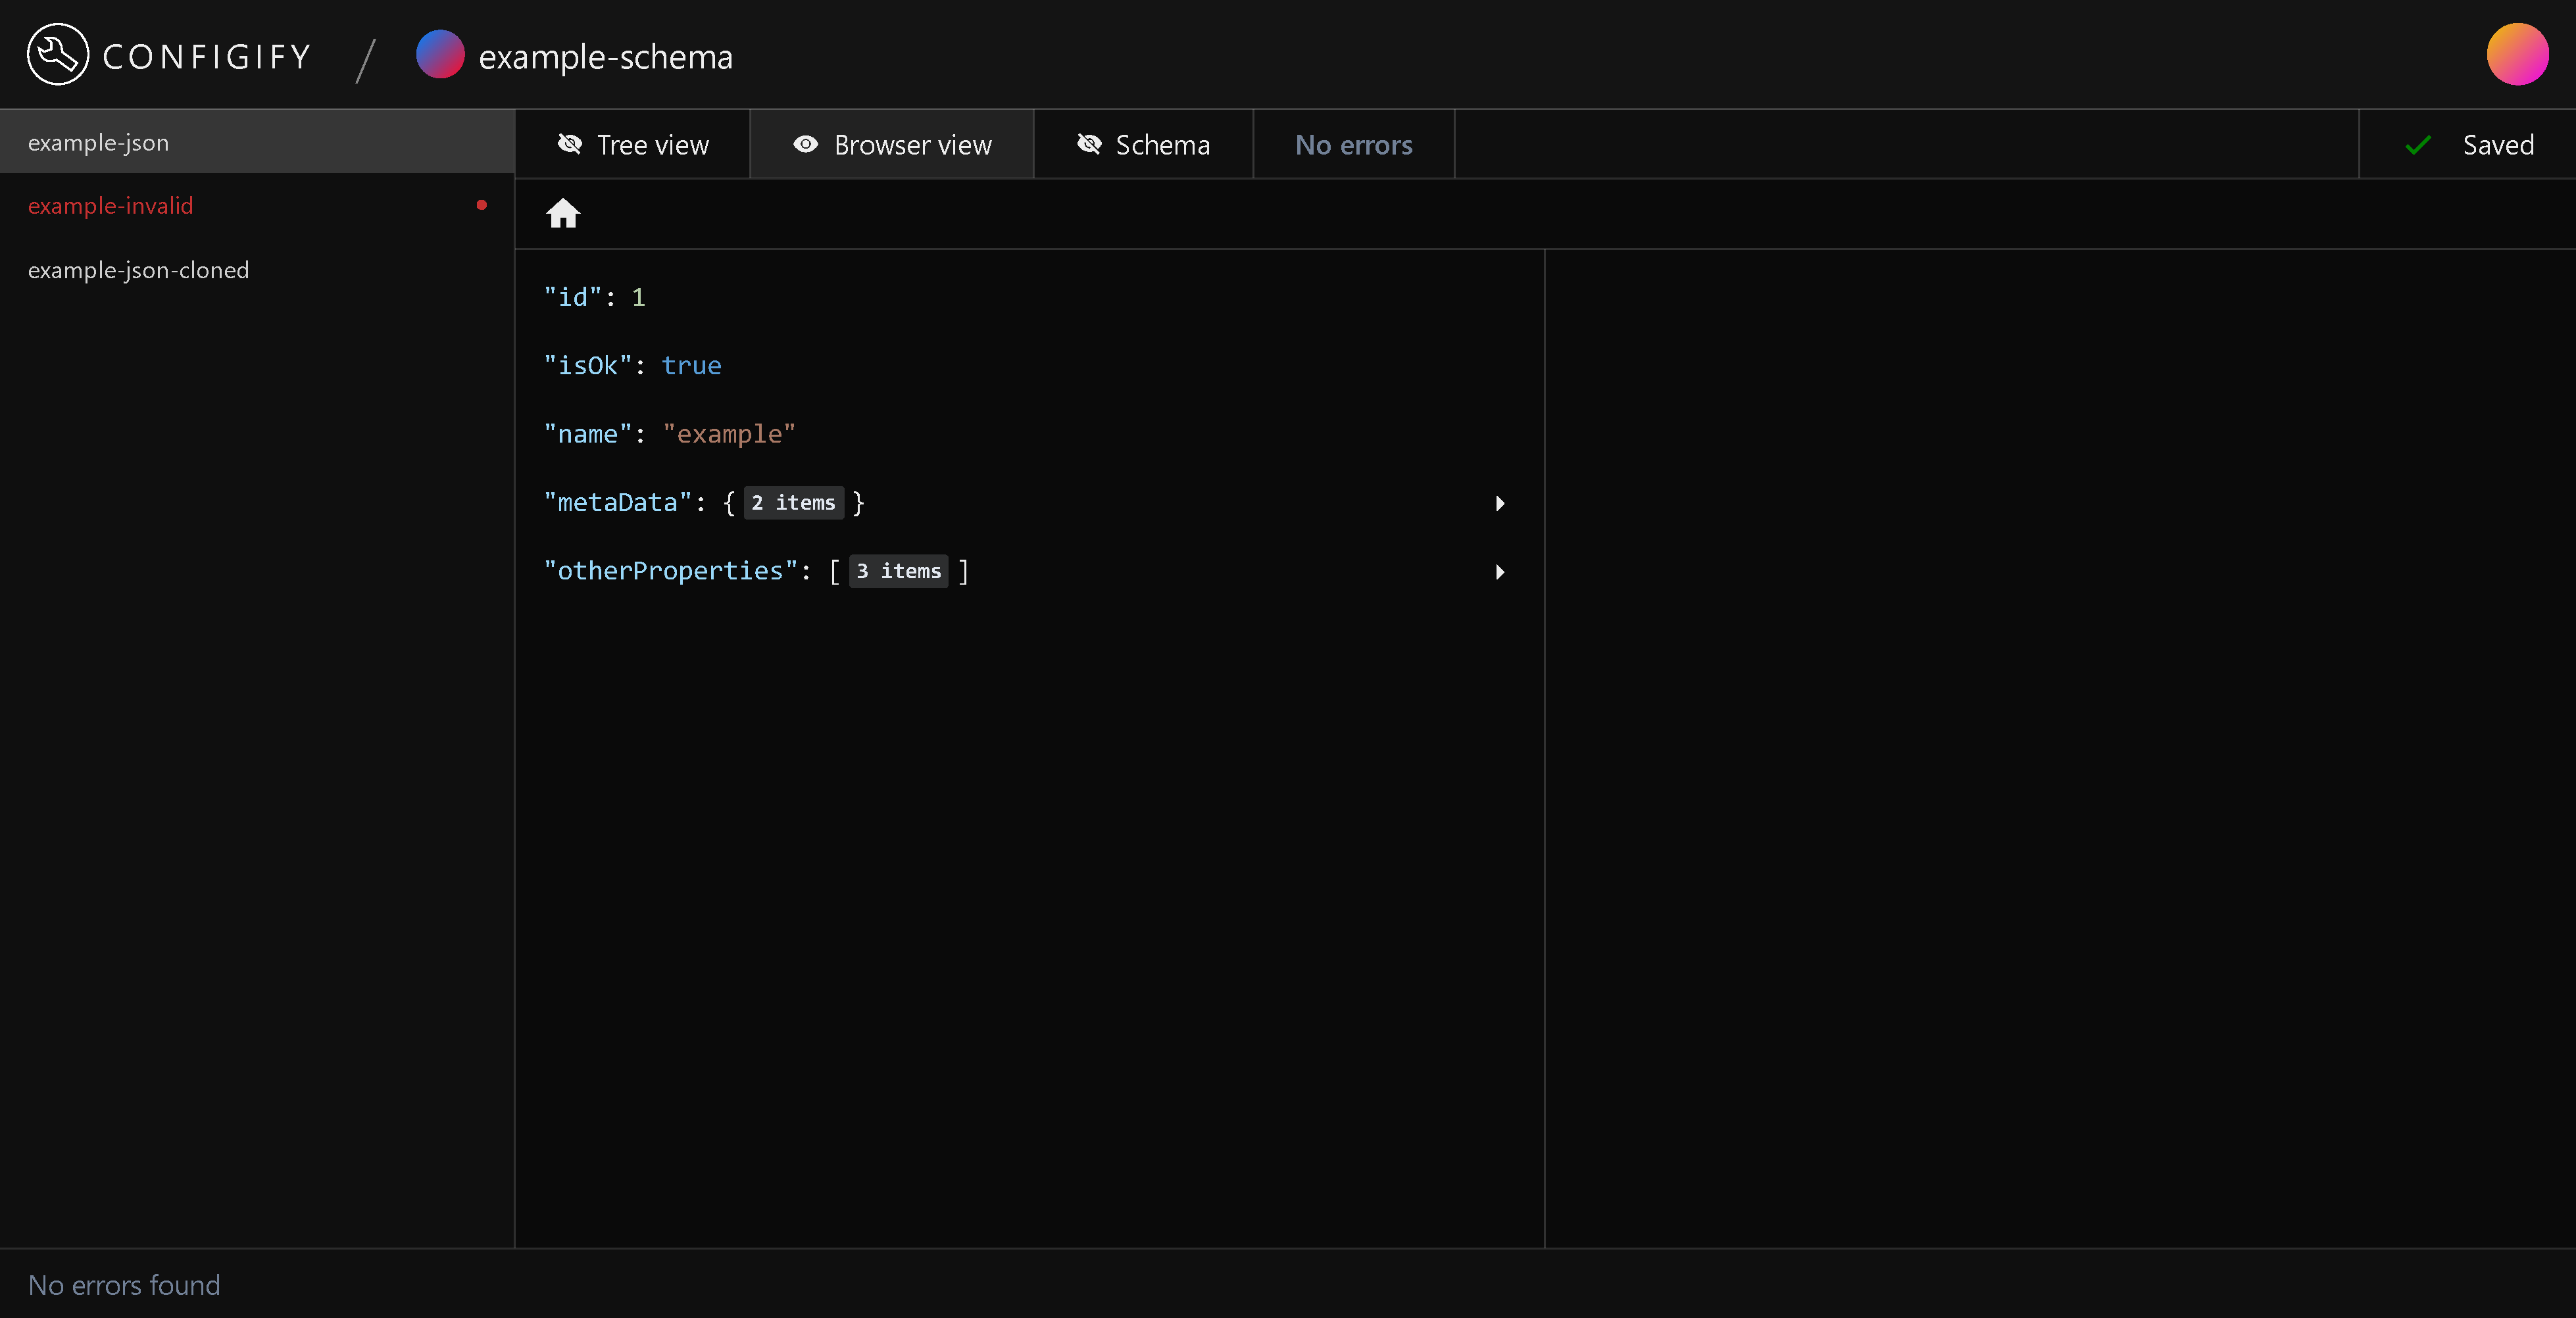
\includegraphics[width=.95\textwidth]{Figures/browser/index.pdf}
     \caption[Configuration Browser Interface]{Illustration of the Configuration Browser Interface}
     \label{browsing:browser}
   \end{minipage}\hfill
\end{figure}

\noindent
The user can switch between the configuration browser and the Tree view. Its also possible to view the schema. In the left pane, one can see a list of all the other configurations for the template. It's possible to click any one of these to quickly switch configuration. The title of these are also highlighted as red if the configuration is marked as invalid. This allows the user to quickly navigate through all the configurations to fix any error.
\begin{figure}[!ht]
   \begin{minipage}{1\textwidth}
     \centering
     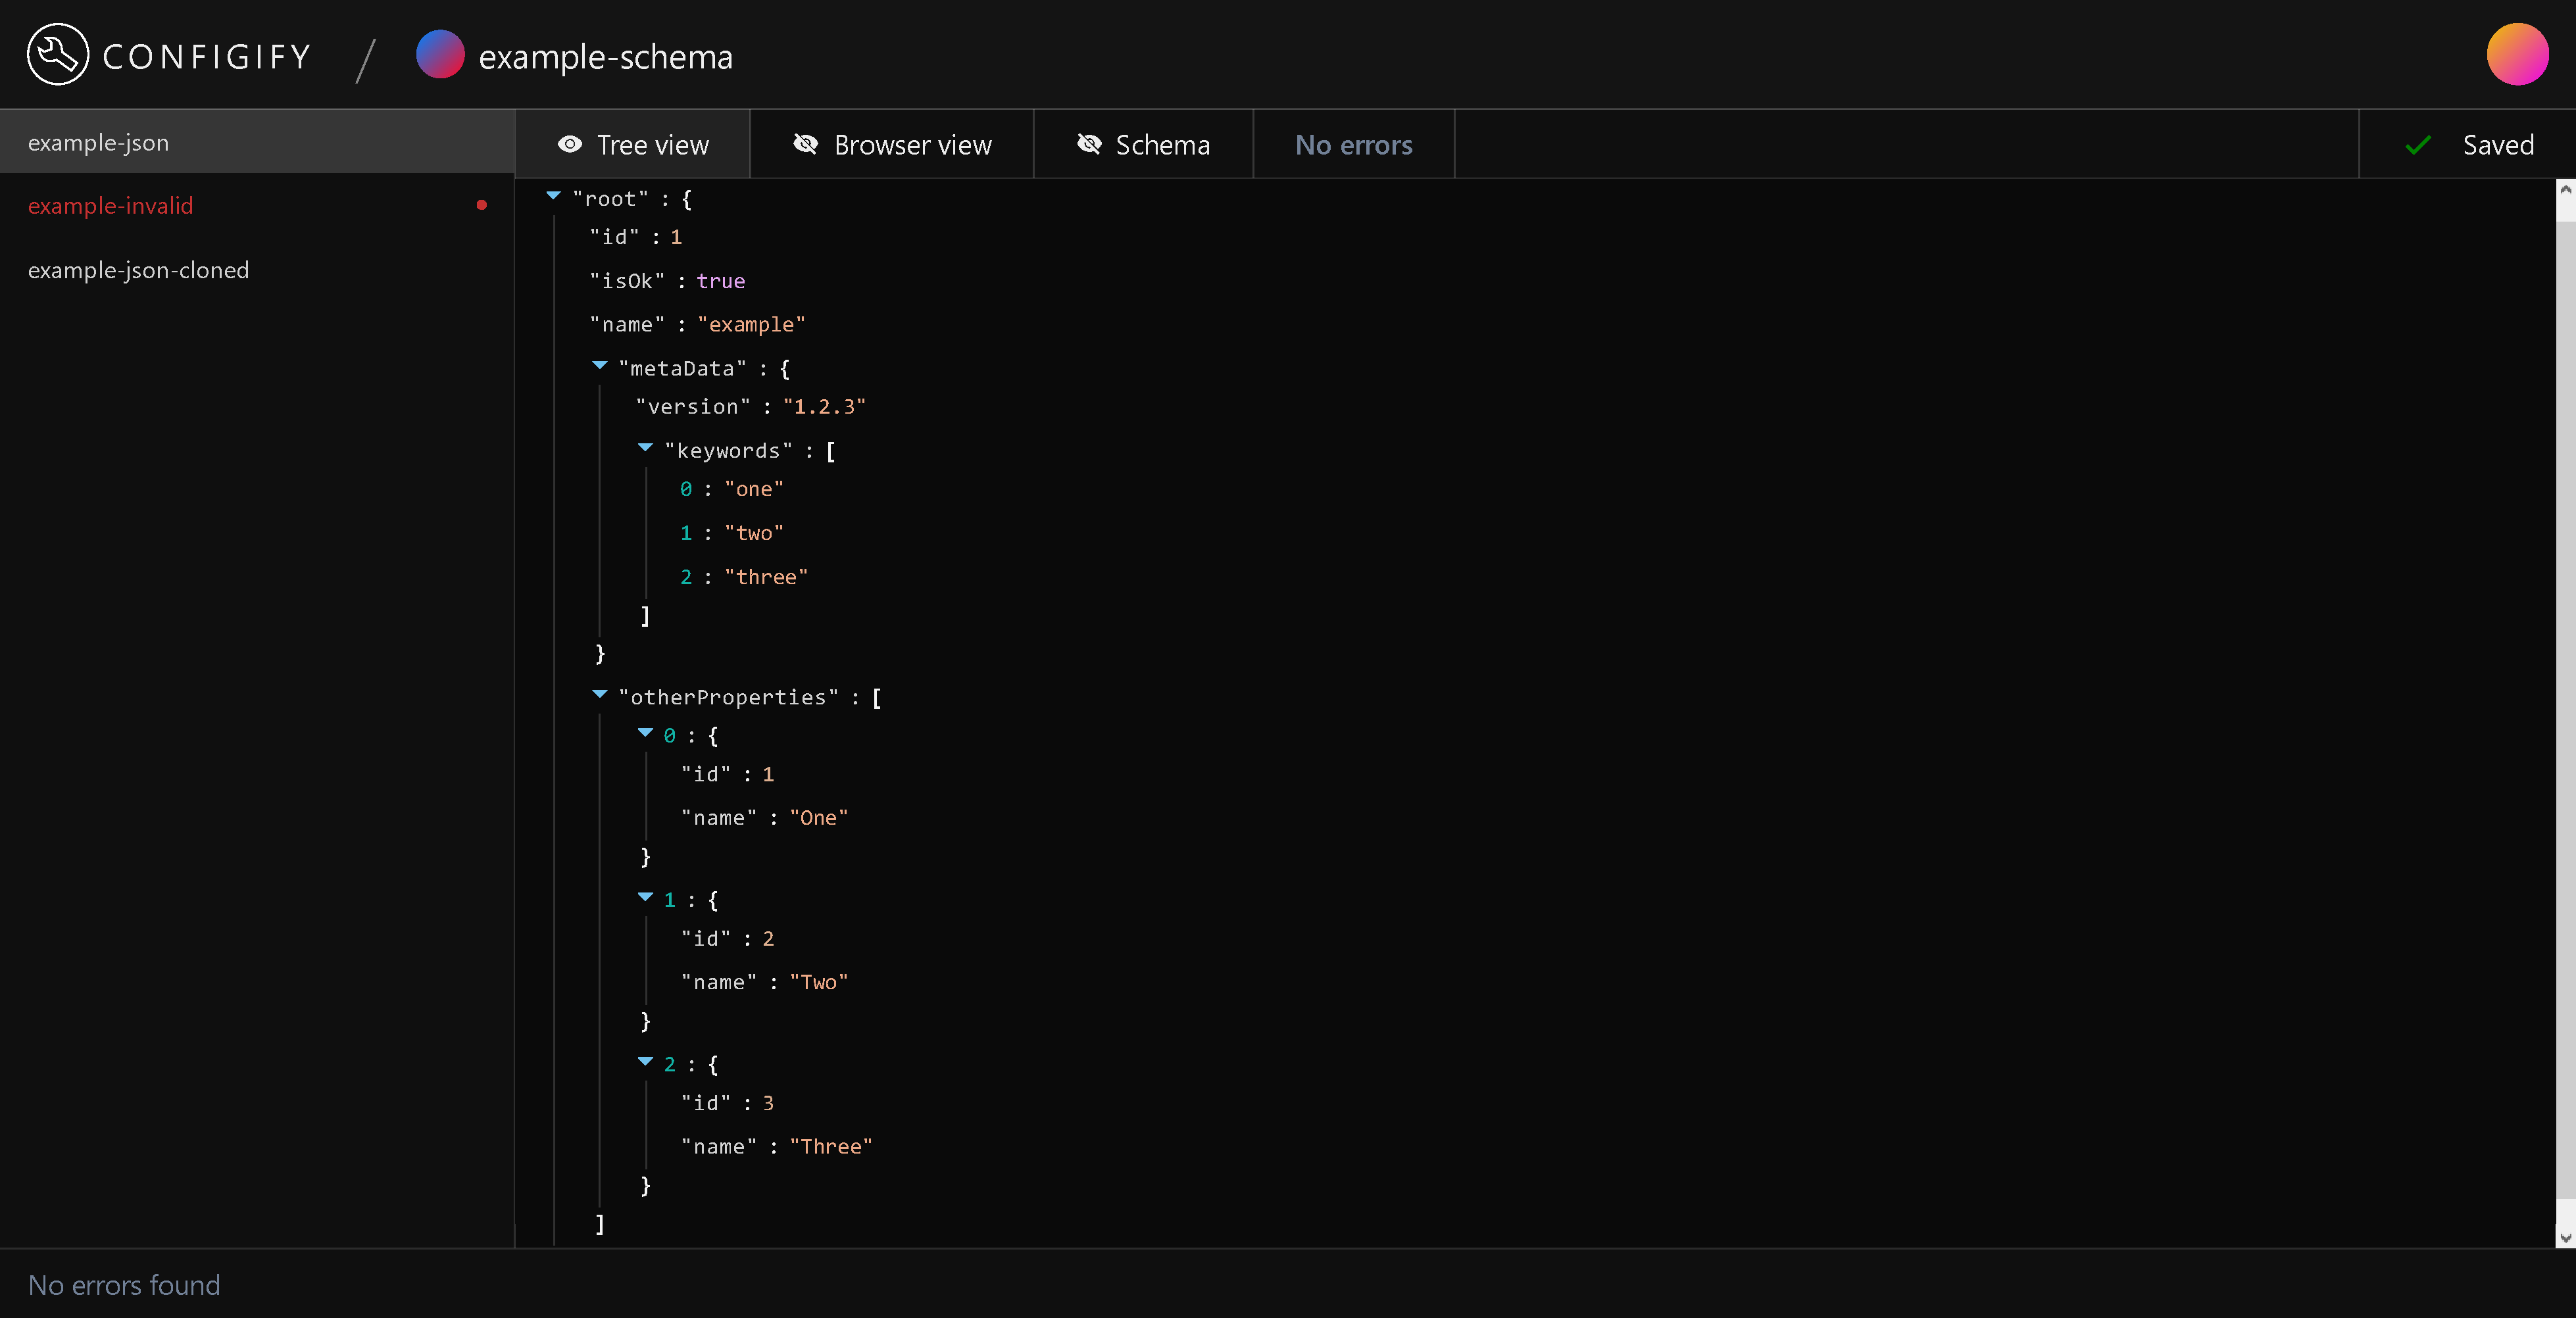
\includegraphics[width=.95\textwidth]{Figures/browser/index-treeView.pdf}
     \caption[Configuration Browser Interface, Tree view]{Illustration of the Configuration Browser's Tree view}
     \label{browsing-treeView:browser}
   \end{minipage}\hfill
\end{figure}

\subsubsection{Descending the object tree}

The user can explore the object tree of the JSON file by clicking on any of the fields that contain objects. This action will display the content of that object in the right pane. As JSON objects can contain unlimited nested objects, clicking an object in the right pane that contains more objects will hide the original main pane, and the right pane will be shifted to the left to display the new content.

\begin{figure}[!ht]
   \begin{minipage}{1\textwidth}
     \centering
     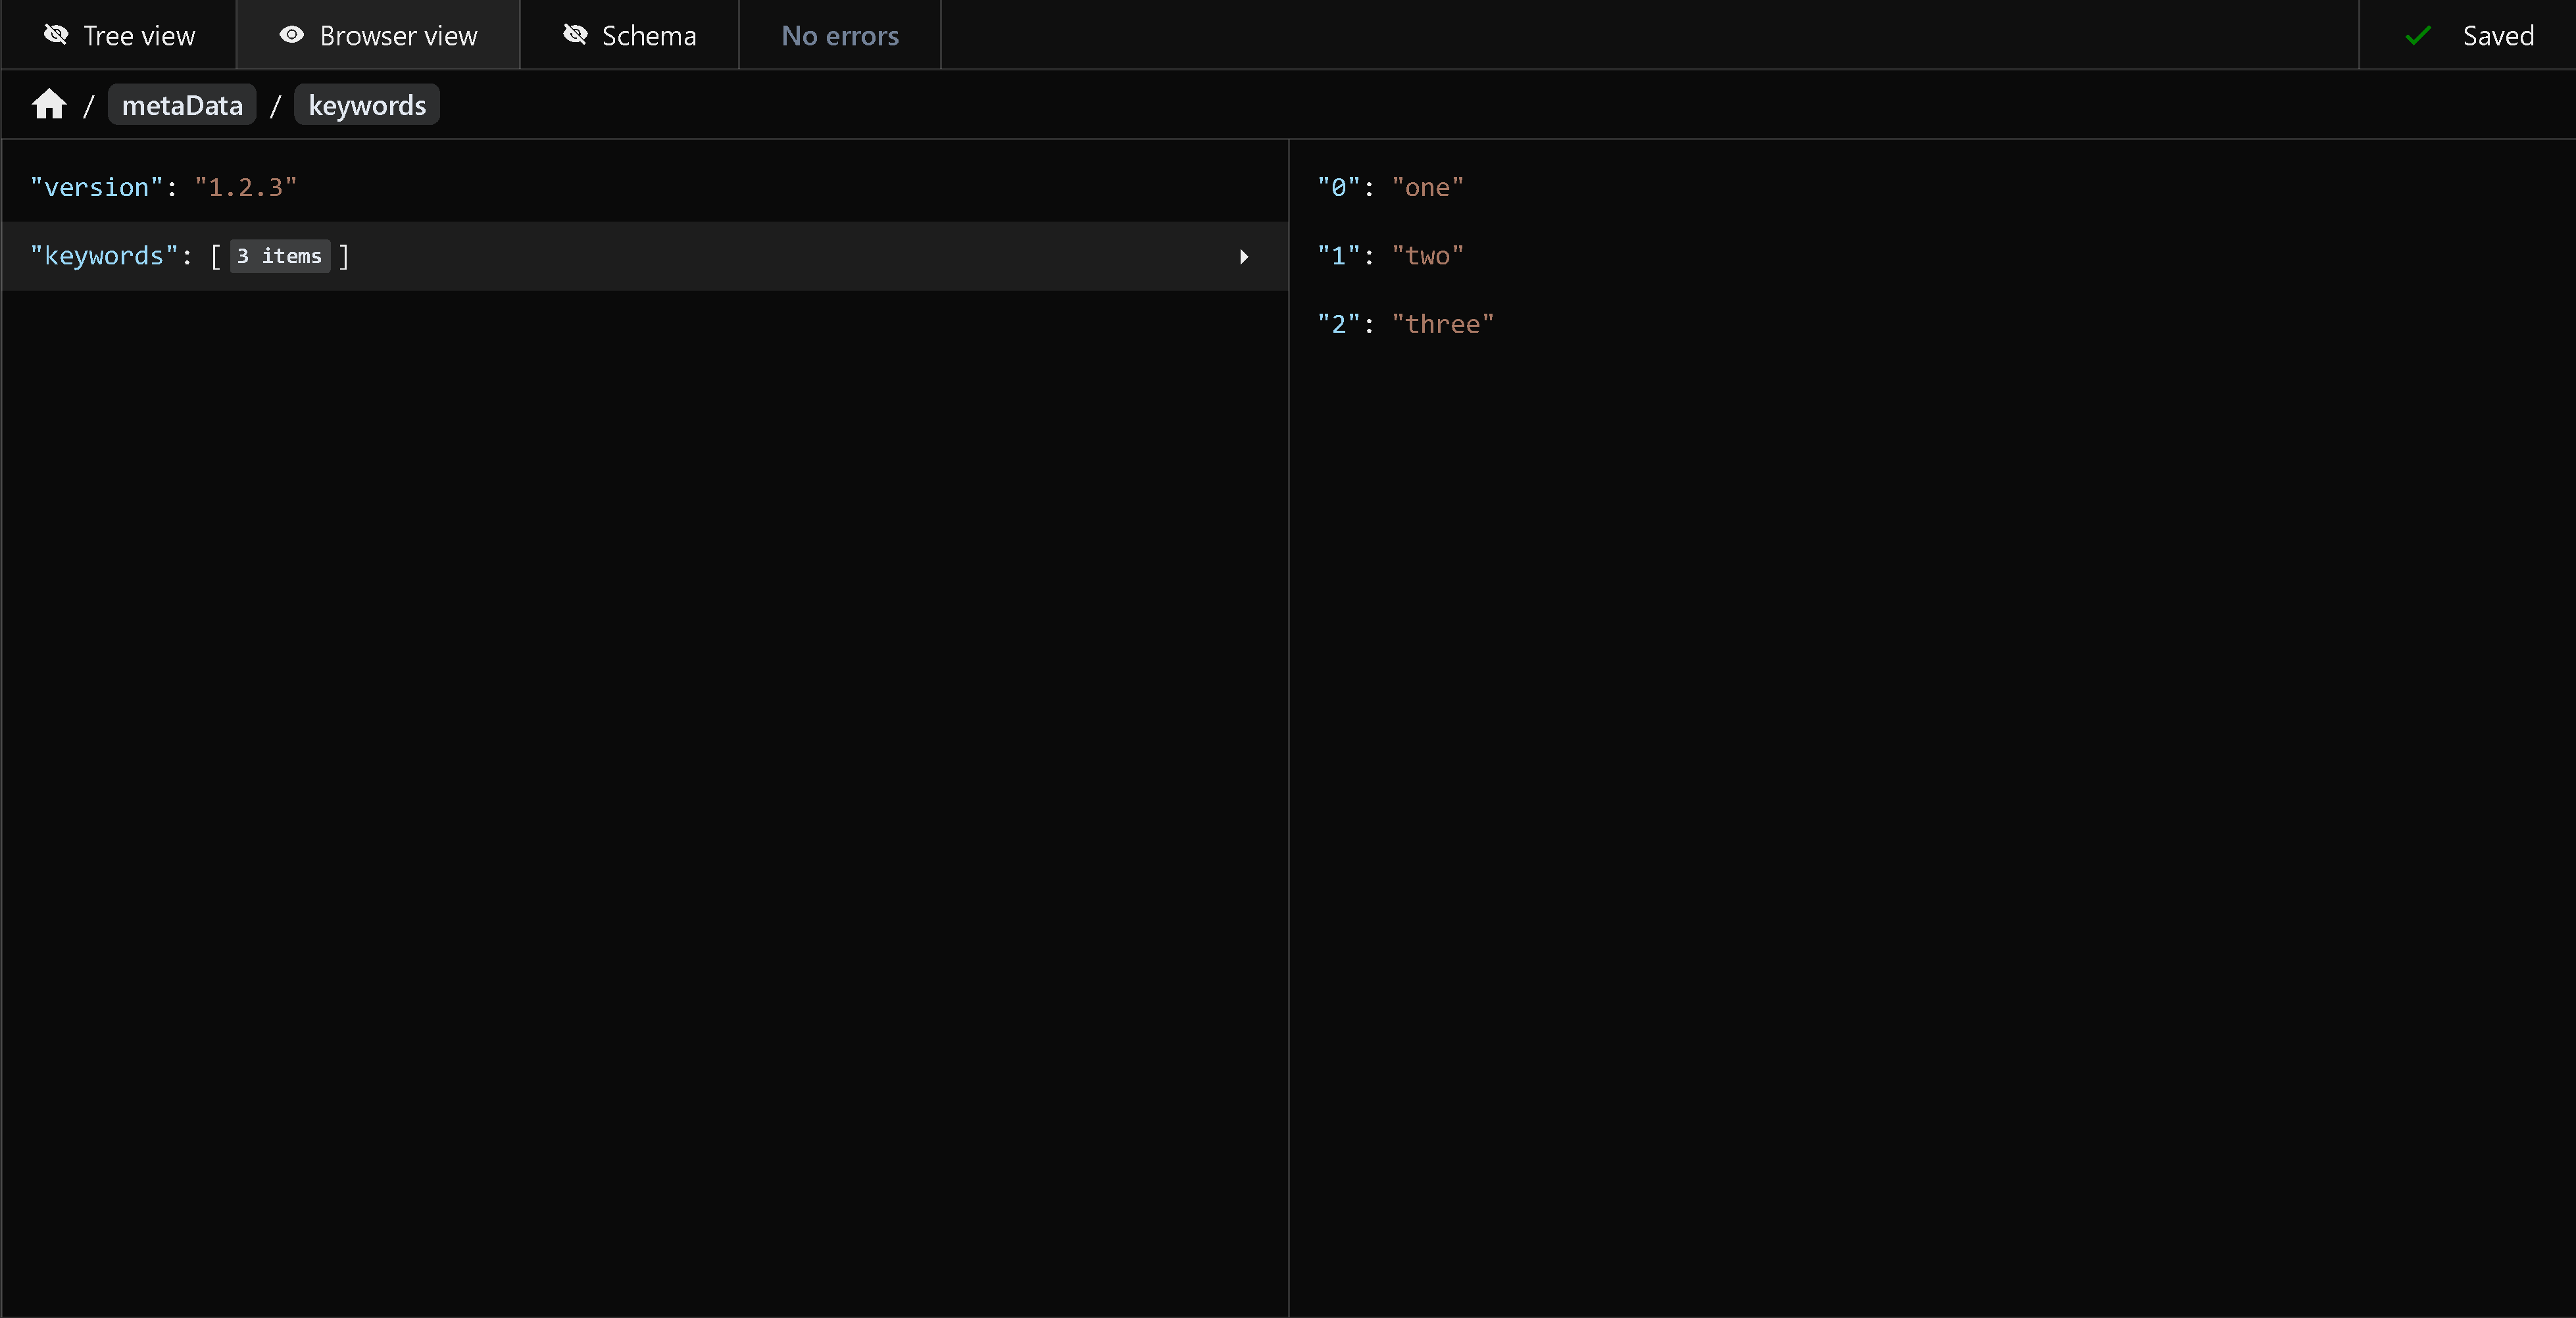
\includegraphics[width=.95\textwidth]{Figures/browser/descending-crop.pdf}
     \caption[Configuration browser navigation]{Screenshot of the Configuration Browser navigating through a JSON file}
     \label{descending:browser}
   \end{minipage}\hfill
\end{figure}

\subsubsection{Editing values}

In order to modify or insert values, the user must switch to the Tree view. To make changes to a value, the user will need to hover over the object that they wish to modify. Two buttons will appear, one for editing the field and one for deleting it. Clicking the edit button will display a box containing the existing data. As the user enters new data, they can choose to save it as a string or, if the system detects that it can be inferred as a different data type, a different save button will appear underneath. \\

\noindent 
Example 1:

\noindent 
If the user types '12' in the box, one can either save it as a string, or infer it as a number.\\


\noindent 
Example 2:

\noindent 
If ones writes '\{"id": 1,
"name": "table"\}', the system is able to infer that this text represents an object. It then offers a button to convert the text into an object. See \autoref{editing:browser} and \autoref{editing:browser-object-creation} for a demonstration. \\

\noindent
To add values, one needs hover the mouse over the desired object. A plus-sign will then appear, clicking this allows the user to choose a name for the value. Once it's created, one is able to edit the data as mentioned above. 

\begin{figure}[!ht]
   \begin{minipage}{1\textwidth}
     \centering
     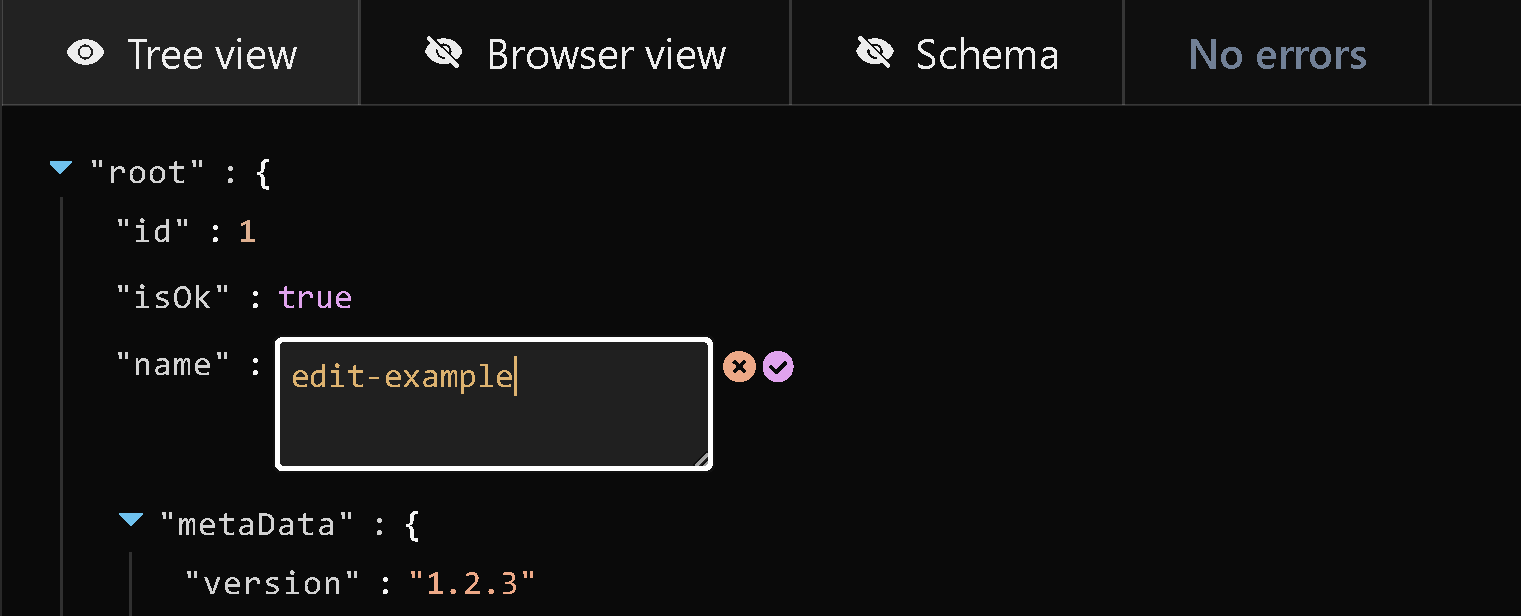
\includegraphics[width=.95\textwidth]{Figures/browser/editing-crop-crop.pdf}
     \caption[Tree view - Edit field]{A figure showing the Configuration Browser’s editing functionality in the Tree view}
     \label{editing:browser}
   \end{minipage}\hfill
\end{figure}

\begin{figure}[!ht]
   \begin{minipage}{1\textwidth}
     \centering
     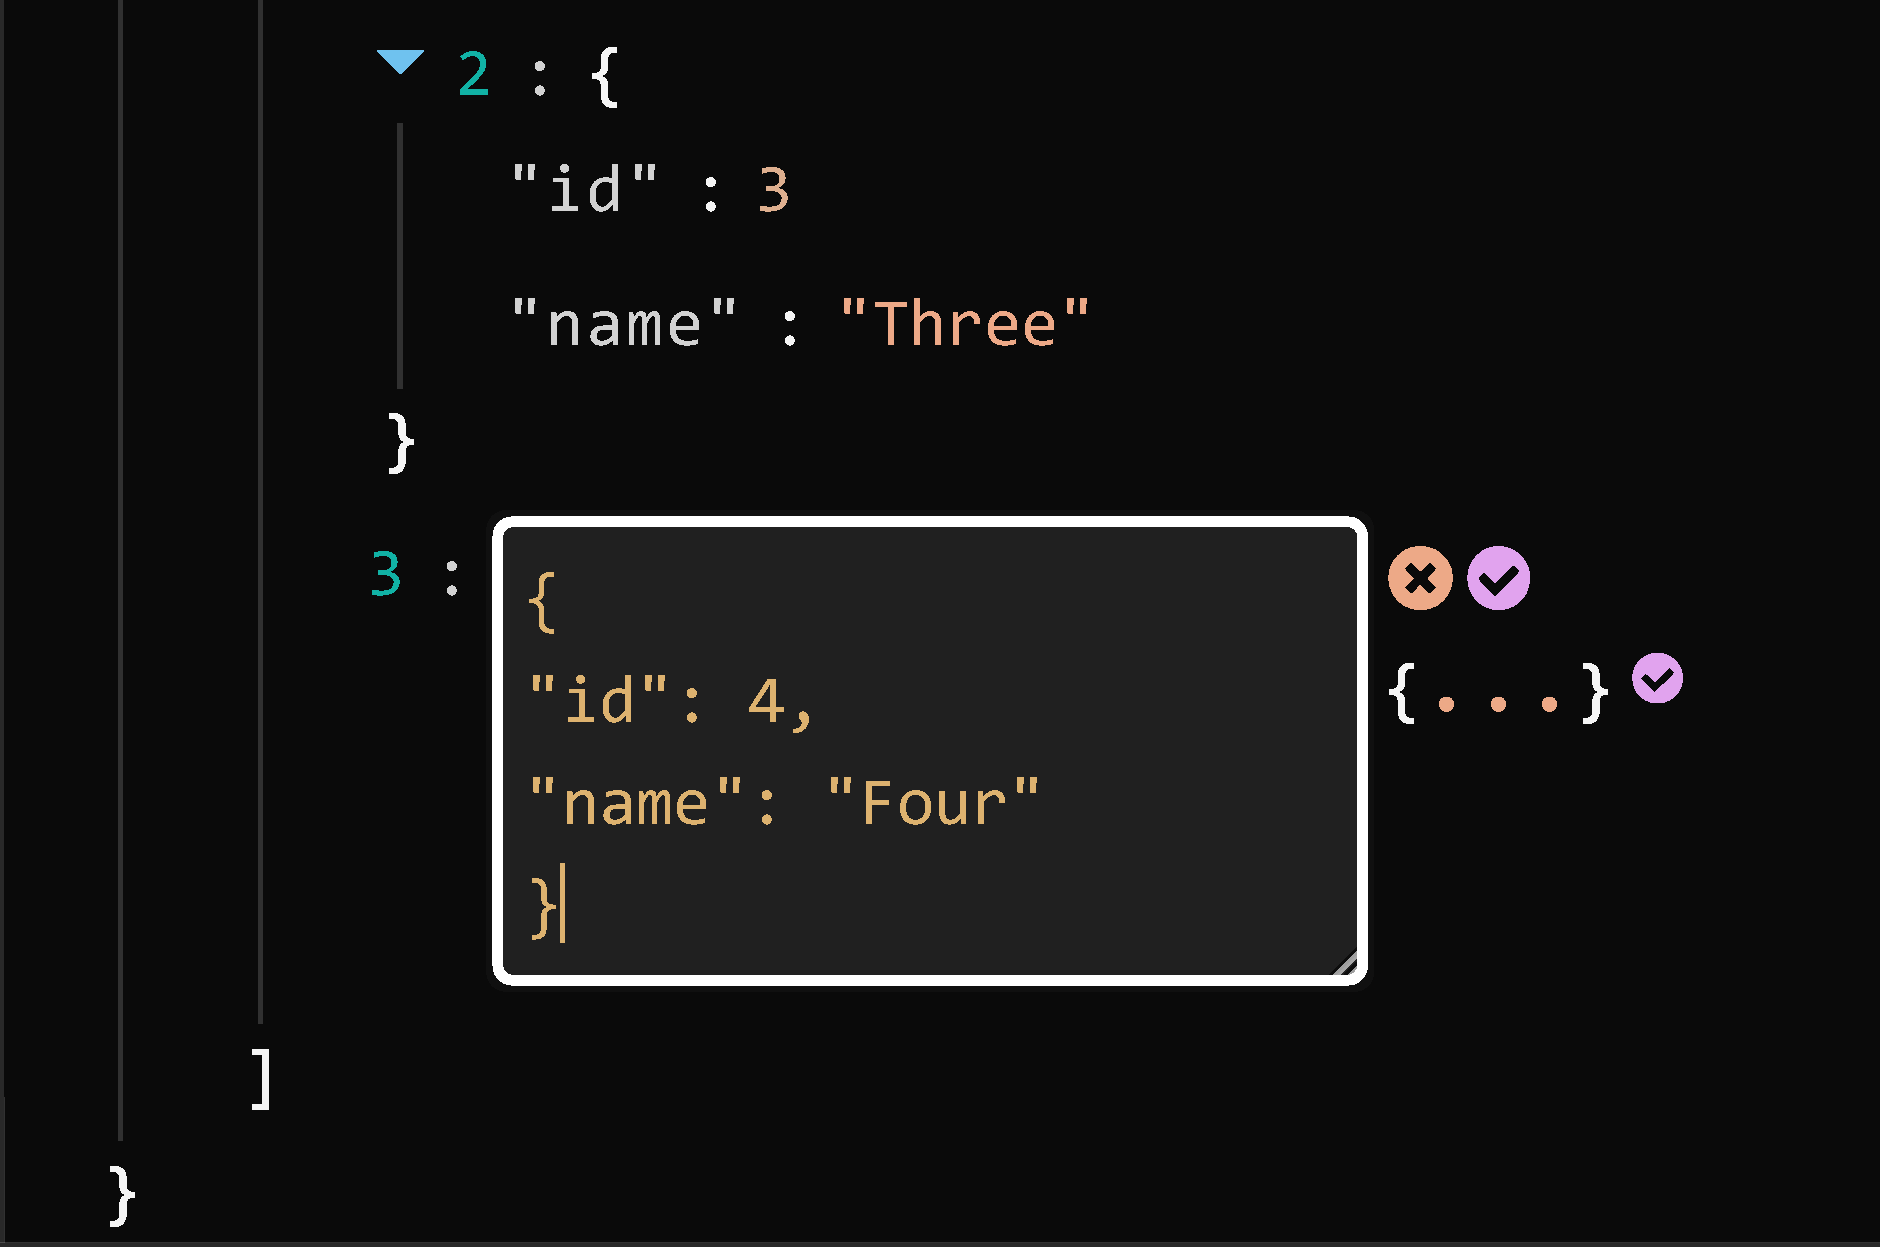
\includegraphics[width=.95\textwidth]{Figures/browser/editing-object-creation-crop-crop.pdf}
     \caption[Adding a complex object]{A figure showing how a user can add a complex object to the configuration}
     \label{editing:browser-object-creation}
   \end{minipage}\hfill
\end{figure}

\subsubsection{Jumping to errors}

In the case of configuration errors, a line at the bottom of the screen will display the total number of errors. This line is interactive and can be expanded to show each error individually. Moreover, if the user is in the browser view, one can simply click on each error to navigate to the location of the error automatically. 

\begin{figure}[!ht]
   \begin{minipage}{1\textwidth}
     \centering
     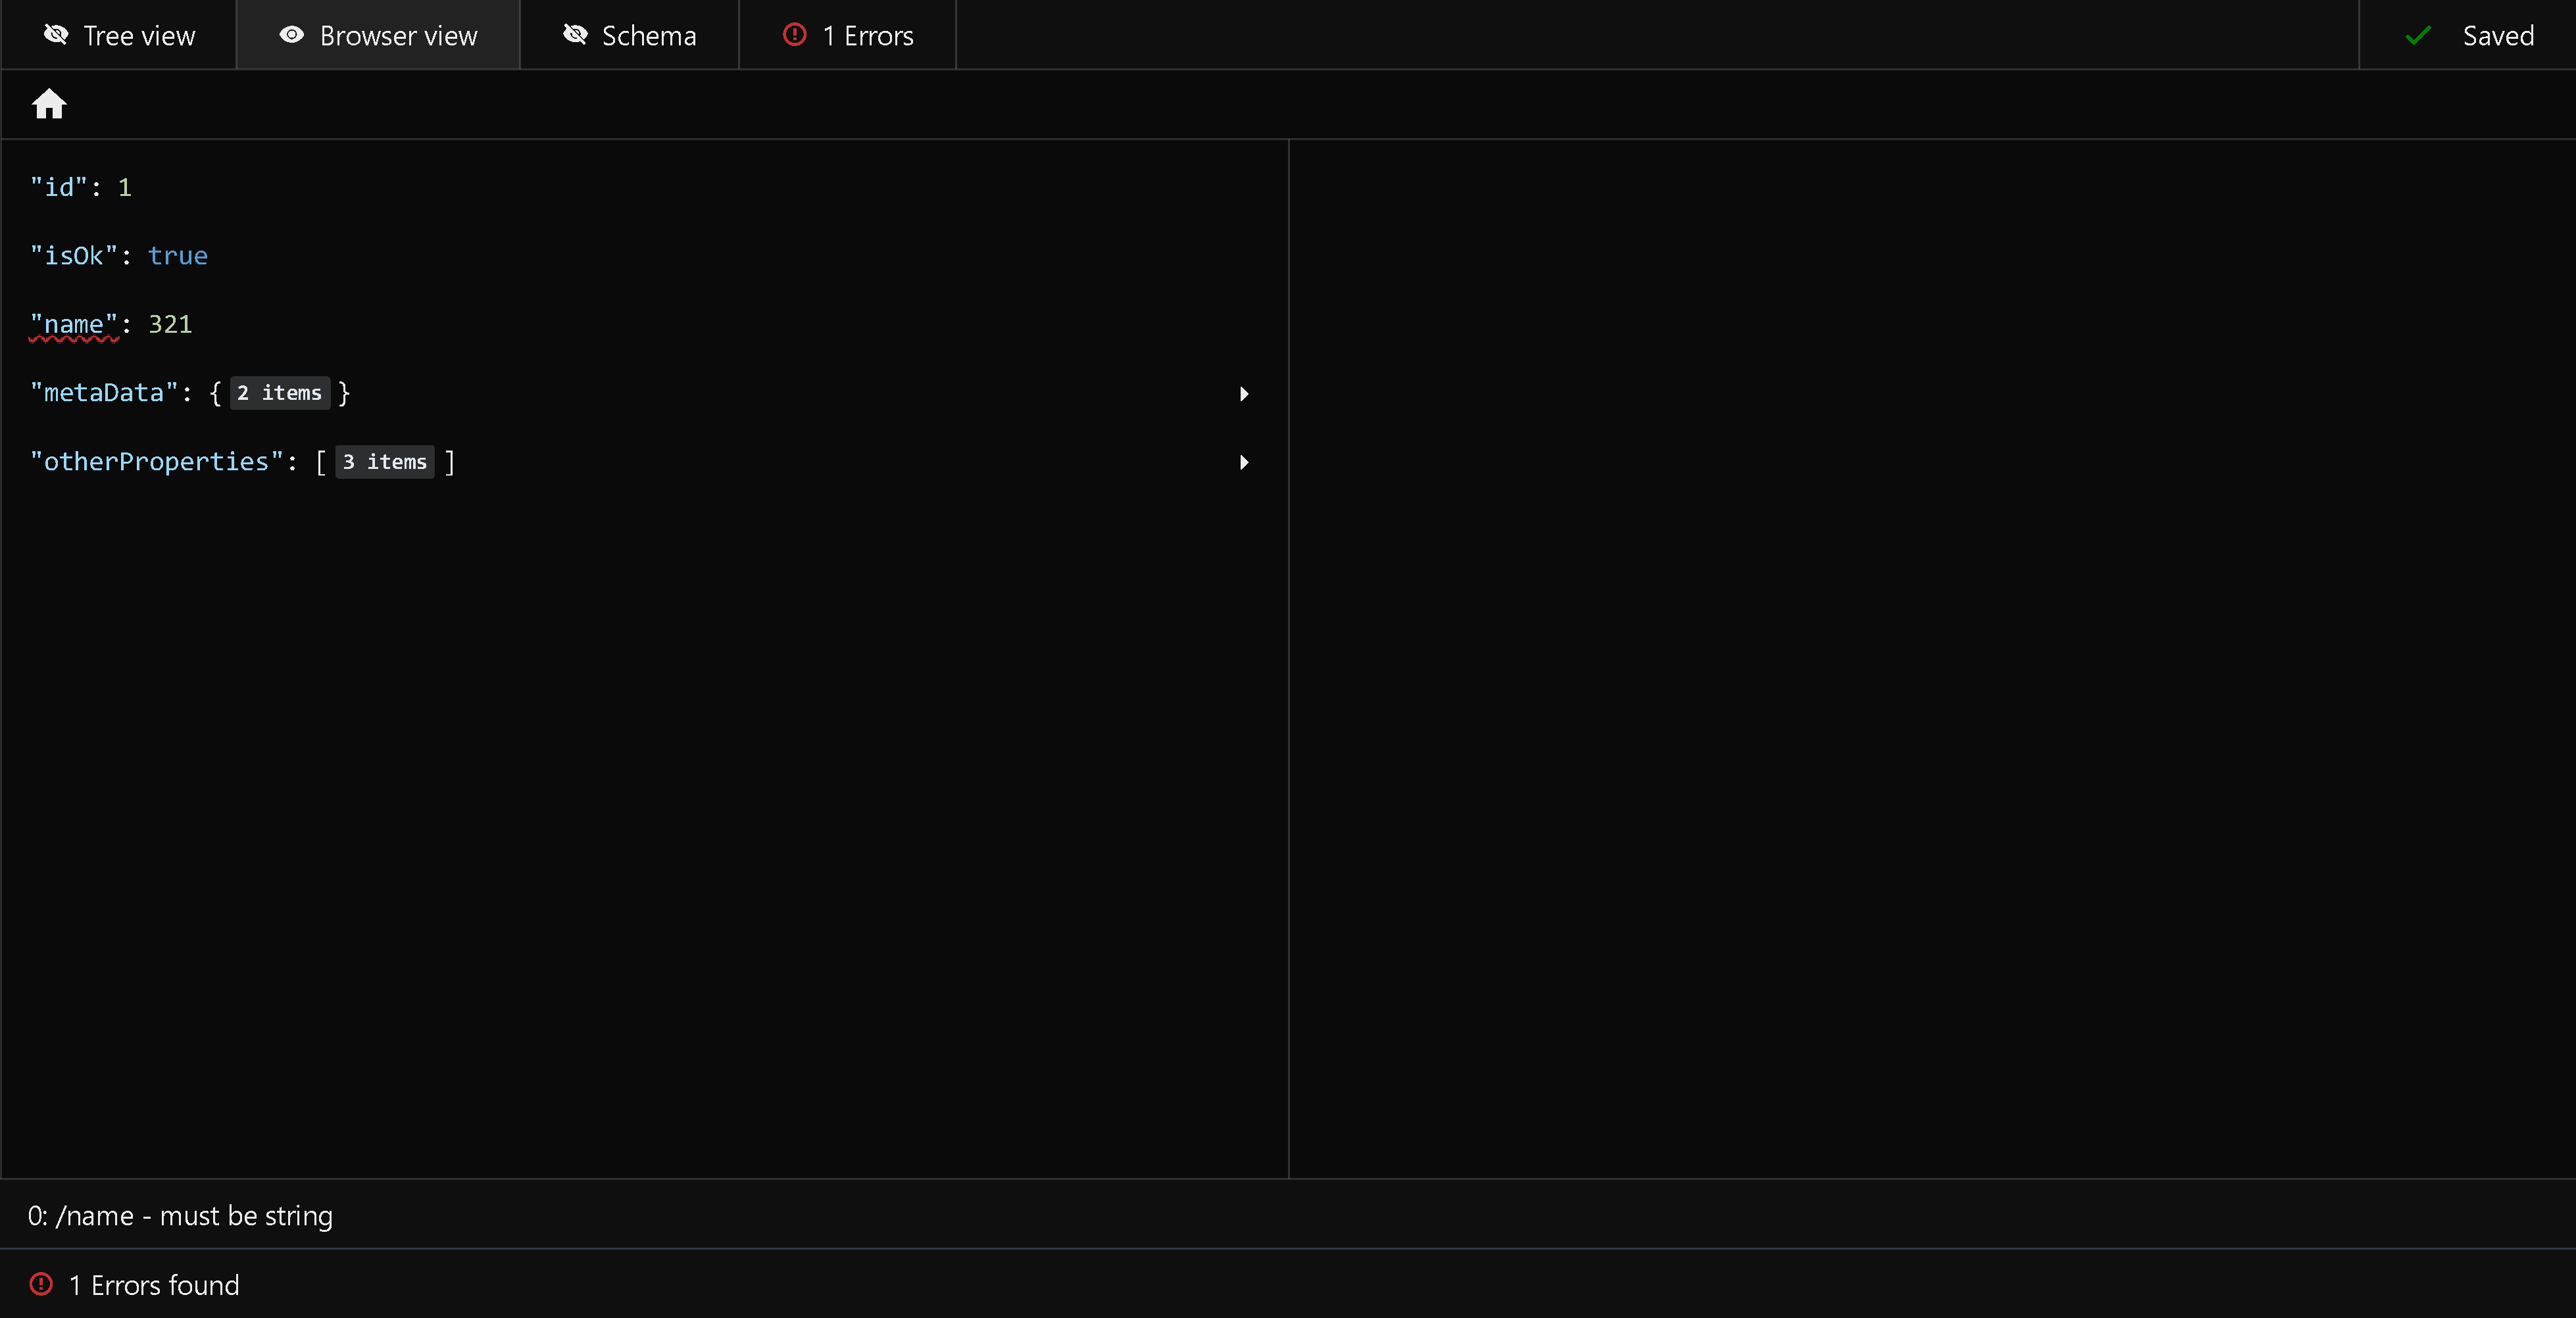
\includegraphics[width=.95\textwidth]{Figures/browser/error-crop.pdf}
     \caption[Error handling showcase]{A figure demonstrating the Configuration Browser’s error handling functionality, with clickable errors leading to their location in the JSON configuration}
     \label{errors:browser}
   \end{minipage}\hfill
\end{figure}

\subsection{Account management}

Account management is a crucial aspect of our project. We have developed a comprehensive account management system that enables users to perform essential functions such as creating, modifying, and deleting their accounts as required. 

\subsubsection{Deletion}

To delete their account, the user must navigate to the account page and click the delete button. A confirmation dialog appears, that once confirmed, makes the server removes all user data associated with the account from the database, and the user is logged out. \autoref{delete:account} \\

\noindent
We have taken appropriate measures to ensure that the deletion process is irreversible. This means that once a user confirms their request to delete their account, all associated data is permanently removed from our system. This approach serves to safeguard user privacy and prevent the retention of user data by our application. 

\begin{figure}[!ht]
   \begin{minipage}{1\textwidth}
     \centering
     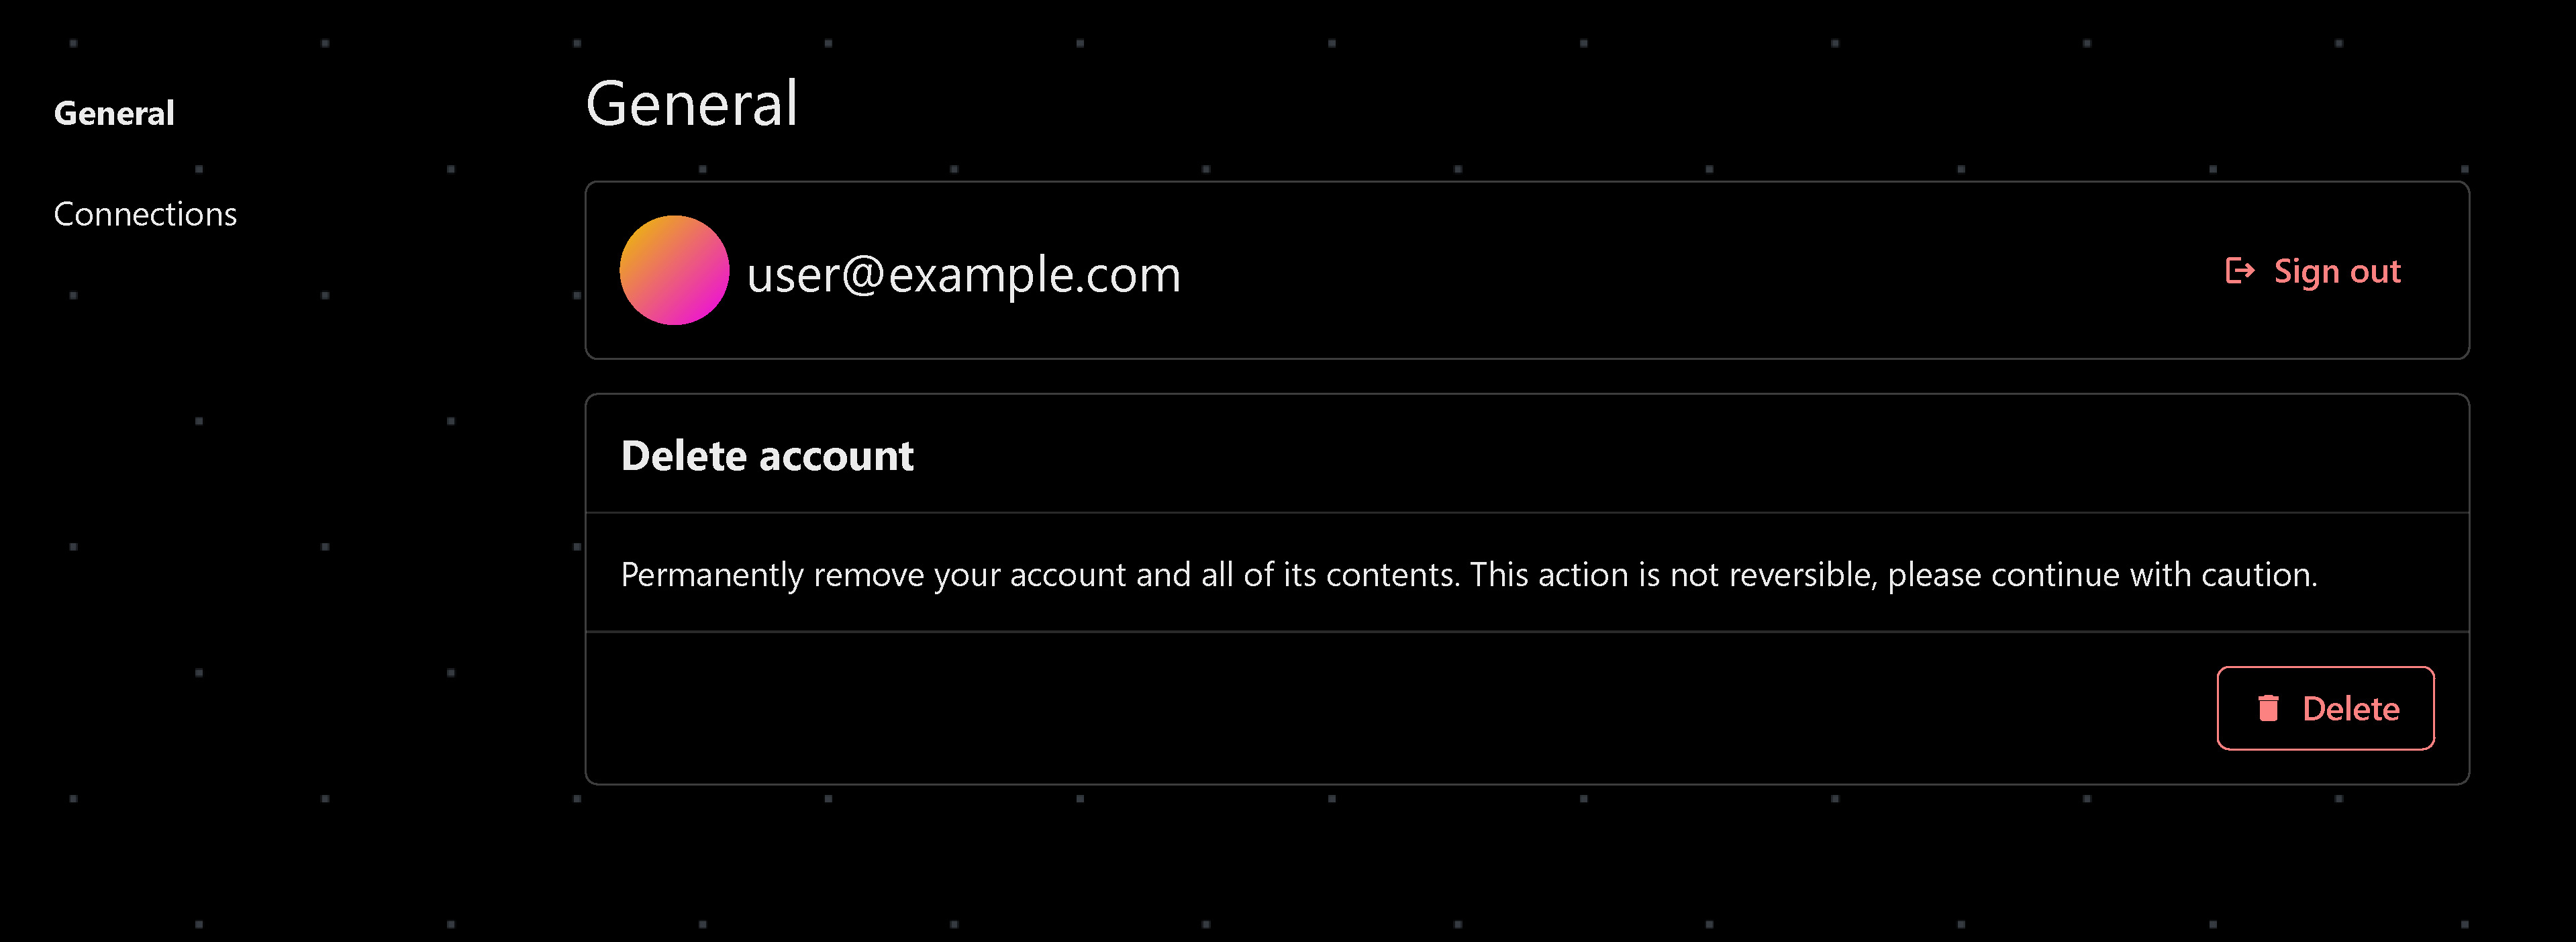
\includegraphics[width=.85\textwidth]{Figures/settings-page/general-settings-page.pdf}
     \caption[Delete account page]{The account page showing the delete functionality}
     \label{delete:account}
   \end{minipage}\hfill
\end{figure}

\subsubsection{Connection}

As one of the main requirements was the ability to link accounts, we have developed and integrated functionality that enables users to register or log in using their preferred identity provider and subsequently link their accounts that share the same email address. \\

\noindent
Users can manage their account connections via the dedicated connections page, where they are able to view their current connections, establish new connections with additional identity providers, and remove existing connections as desired. The connections page showing an account that is linked to Google and email but not GitHub can be seen in \autoref{connections:account}

\begin{figure}[!ht]
   \begin{minipage}{1\textwidth}
     \centering
     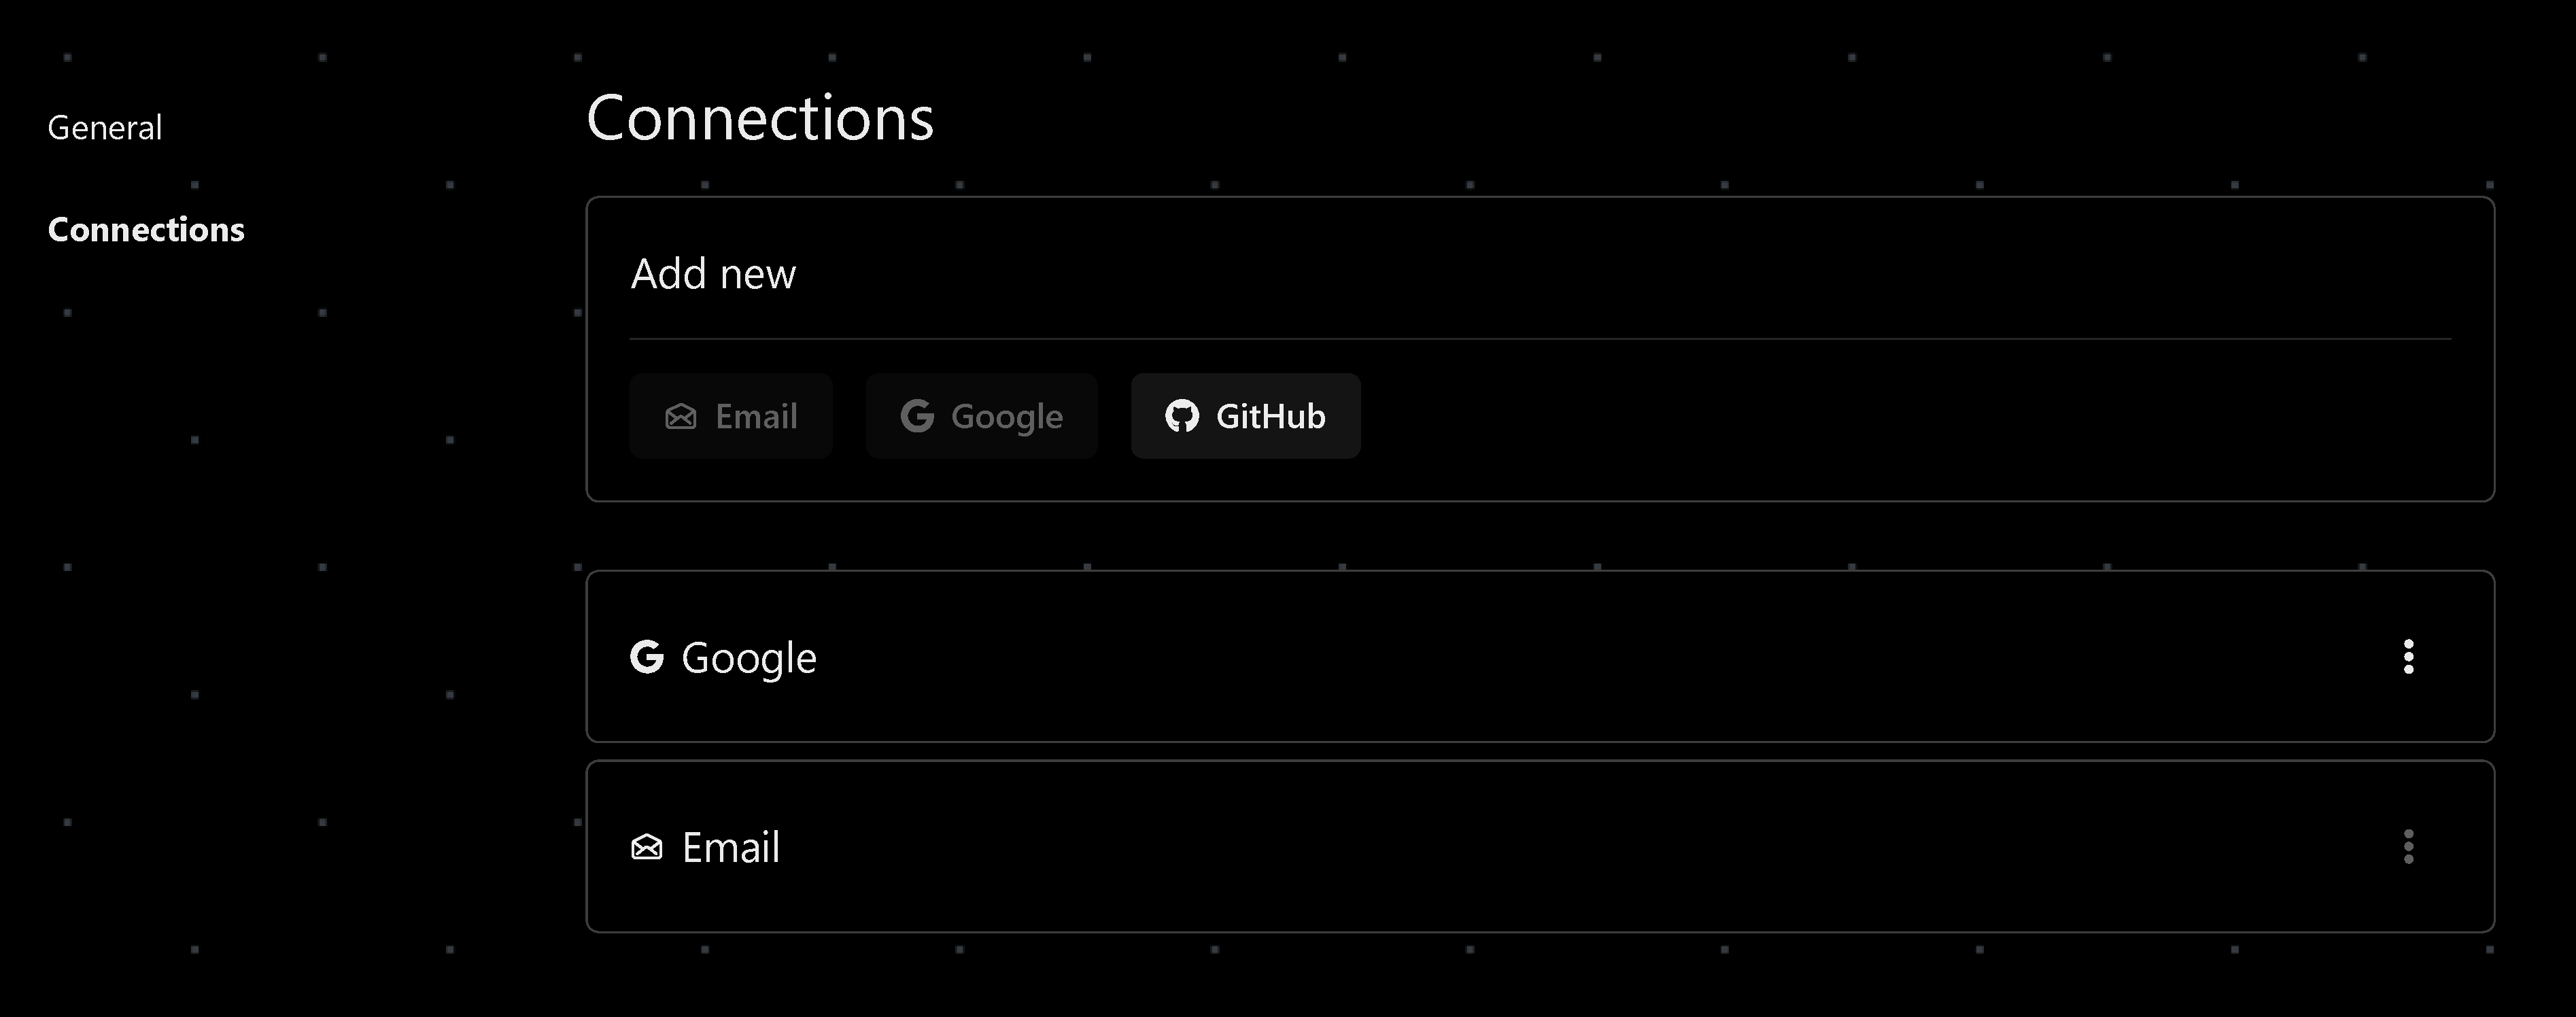
\includegraphics[width=.85\textwidth]{Figures/settings-page/connections-page.pdf}
     \caption[Connections page]{The connections page}\label{connections:account}
   \end{minipage}\hfill
\end{figure}

\subsection{Endpoints}

\subsubsection{Validate}

This public endpoint takes in a JSON schema and a JSON as a string, then validates the JSON against the given schema as requested by the client. The validation process determines whether the JSON is valid or invalid based on the given schema. If the JSON is invalid, the endpoint will return an array of errors and paths to the errors. 

\subsection{Database}

% This is the short description, we can maybe move that part out of the Appendix if the report is too short 

Our database schema was designed using the Prisma ORM. It's written as a Prisma schema and consists of five tables: Account, Session, User, Template, and Configuration. The schema was optimized for NextAuth and allowed for easy authentication and authorization. The configuration model was designed to store JSON templates and configurations, which could be edited by the user. The solution was effective and allowed for efficient database management and usage. \\

\noindent
The complete database schema is presented in a figure in the appendix, as shown in 
\autoref{database:schema}.
Additionally, a detailed description of the database design can be found in the \hyperref[chap:database-schema]{database section of appendix E, System documentation}. 

%%%%%%%%%%%%%%%%%%%%%%%%%%%%%%%%%%%%%%%%%%%%%%%%%%%

\section{Administrative results}

\subsection{Work in Jira}

Jira was successfully utilized to keep track of the progress and backlog of the project. Jira provided a good system for splitting the project into smaller tasks, making it easy to get started working as you knew exactly what you were going to work on. 

\subsection{Sprints and planning} 

% - We didn't estimate time needed for issues (planning poker) so no burndown charts \\

\noindent
During the course of our project, we encountered some challenges with our sprints and planning. One issue was that our team did not estimate the time needed for Jira issues or do planning poker like we planned. This made it difficult to accurately plan and allocate resources for each sprint. \\

\noindent
Additionally, while the team members who were focused on coding were able to make progress, the member assigned to the scrum master duty rarely showed up to our daily work meetings and did not perform his assigned duty. This lack of participation from a key team member hindered our ability to effectively plan and execute our sprints. Although the rest of the team should have recognized and resolved this issue, it went unattended as their focus was consumed by tasks aligned with their individual responsibilities. \\

\noindent
As a result of these challenges, we were unable to generate burn-down charts to track our progress. This made it difficult to assess our progress and adjust our plans accordingly. \\

\subsection{MVP}

During the development of our app, we found it important to prioritize the MVP functionality over the stretch goals. This allowed us to prioritize and deliver the most important features first, while ensuring that the product met the needs of our client. 

% \subsection{Time lost due to INGA2300}

% Section commented out on the request of our supervisor 

% During the first months of this semester, we had to spend a lot of time working on a different subject, INGA2300. This was a group project, where we had to work together with another bachelor's group from a different study. We had to spend a lot time researching in this subject, as we were required to create a hypothetical solution to a climate problem. We were then required to write an extensive report at the end, and together with a lot of mandatory assignments and preparation for the exam, we didn't have as much time during this period, as we would have wanted.

% During the initial months of the semester, our focus was directed towards a different subject, INGA2300. This entailed a collaborative project with another bachelor’s group from a separate field of study. Our task was to devise a hypothetical solution to a climate issue through extensive research. The culmination of this project was an elaborate report. Coupled with mandatory assignments and exam preparations, our time was considerably constrained during this period.